\chapter{多视角人脸数据采集方案设计与实现}
\label{chap:platform}

为产出高质量的内容,影视、游戏等行业对高逼真3D人脸模型的需求日益增加,
能从现实世界中重建模型的3D人脸重建技术受到了广泛关注。
然而,可用于实现人脸几何和材质细节高精度重建的解决方案通常价格高昂,实施困难,其采集的数据往往也由于商业价值较高而不被公开。
本章提出了一套在较为有限的经济和时间成本下实现的多视角人脸数据采集方案。
该方案除了成本较商业方案显著更低外,
其在设计时考虑到后续研究工作所需的灵活性和可扩展性,并尽量使用可在市面上购买的部件,以减少对硬件相关专业知识的需求。
同时配合一些定制的软件和硬件,实现对各个部件的高效统筹控制,为高精度重建所需的数据采集、标定全流程提供支持。

\section{总体目标}

在功能上,本采集方案的目标是提供基于物理的多视角3D重建算法所需的所有数据,
包括相机拍摄的图像,相机和环境光照的标定数据。
这些数据应尽可能准确地在计算机中还原整个采集过程中相机成像的物理过程。
为实现该目标,本方案包括以下几个部分:
\begin{enumerate}
\item 用于固定相机、灯光的机械结构。需要结构稳固,且能容纳足够数量的设备。
\item 相机、灯光的控制设备。能在精确的时间点触发相机快门和闪光灯闪光。
\item 用于照片拷贝、整理的软件。由于相机数量多,需要专门的方案以提升操作效率,并对接后续标定等算法流程。
\item 相机内外参标定方案。用于准确获取相机焦距等内参以及相对位置等外参。
\item 环境光照标定的方案。可用于基于物理光线传播模型估计人脸材质。
\item 采集过程中人工操作的标准操作流程。用以保证采集数据的质量。
\end{enumerate}
本文在设计该采集方案时,除了以上功能性目标外,还主要考虑了以下非功能性目标:
\begin{itemize}
\item 低硬件专业技能需求。本项目作为软件学院的个人项目,其所能得到的机械、结构、电子等方面的专业技术支持非常有限。
因此,为了能在有限的时间内完成该项目,本文尽可能地使用市面上可购买的部件,以减少对相关专业知识的需求。
虽然如此,本文还是使用了少量定制的硬件。

\item 高精度。高精度的数据是高精度3D重建的基础。
因此,对误差的控制贯穿于采集流程的各个环节,指导整个采集方案的软硬件设计。

\item 高效。整个系统在使用时,特别是在对被拍摄对象拍照时,应该尽可能地快速,使大规模数据收集成为可能。

\item 灵活。本方案作为一个主要用于研究性工作的采集系统,其需要具有一定的灵活性,以便应对研究中多变的需求。
基本地,该系统应能同时支持被动光源和主动光源的采集,能灵活配置相机和光源的位置和其他相关参数。

\item 可扩展。相比于业界先进的方案,该方案的规模仍然较小。为支撑后续研究,本方案也应适当考虑未来可能的更大规模的采集需求。

\end{itemize}

本方案采集的数据预计可用于多种3D人脸重建算法,例如本文其他部分介绍的基于可微分渲染的逆渲染方法。
同时也可用于如多目立体等传统的计算机视觉算法。

本章的主要贡献在于对该方案各个部分的设计和实现,以及对其性能的评估验证。
本章的剩余内容将具体介绍该方案的各个部分。

\section{方案设计}

\subsection{支撑机械结构设计}

本方案的第一步是将相机和灯光固定在实验场地中,使其在采集和标定过程中保持空间位置不变。
同时,为了灵活性和可扩展性,该方案还应能支持各个设备能以较高自由度,较方便地调整位置。
\begin{figure}
\begin{subfigure}{0.67\textwidth}
    \centering
    \begin{tikzpicture}[
        node distance=.5cm and .5cm,
        every node/.style={anchor=south west, minimum height=0.8cm, draw, outer sep=0},
        cam/.style={minimum width=1.2cm, fill=brown!20},
        light/.style={fill=brown!20},
        support/.style={fill=blue!30},
        support_layer/.style={fill=blue!15},
        diffuser/.style={fill=gray!20},
    ]
        \node [support, minimum width=7.2cm] (A) at (0,0) {相机支架基座};
        \node [support_layer, minimum width=2.4cm] (layer1) at (0,1) {高度层};
        \node [support_layer, minimum width=2.4cm, right=0 of layer1] (layer2) {高度层};
        \node [cam] (camera1) at (0,2) {相机};
        \node [cam, right=0 of camera1] (camera2) {相机};
        \node [cam, right=0 of camera2] (camera3) {相机};
        \node [cam, right=0 of camera3] (camera4) {相机};
        \node [cam, minimum height=1.8cm] (camera5) at (layer2.south east) {相机};
        \node [cam, right=0 of camera5, minimum height=1.8cm] (camera6) {相机};
        \node [draw=none, above=2.2cm of A] {相机支架};

        \node [support, minimum width=3cm, right=of A] (B) {灯架};
        \path (B.south west) ++(0,1cm) node [light, minimum width=3cm] {摄影灯/闪光灯};
        \path (B.south west) ++(0,2cm) node [diffuser, minimum width=3cm] {柔光箱};
        \node [draw=none, above=2.2cm of B] {灯支架};
    \end{tikzpicture}
    \caption{硬件拓扑结构}
    \label{fig:frame_topo}
\end{subfigure}\hfill%
\begin{subfigure}{0.3\textwidth}
    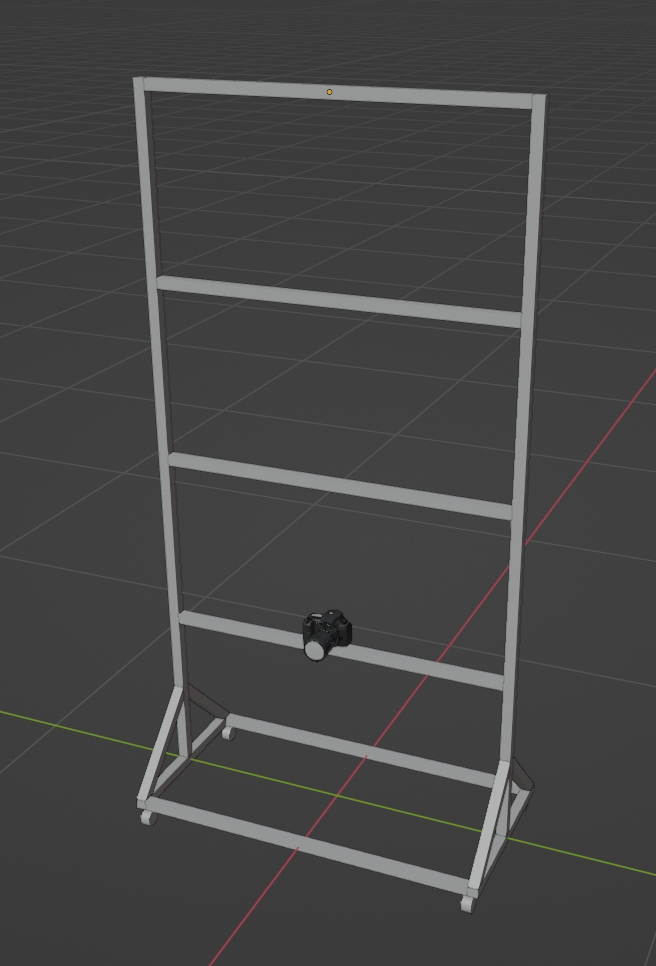
\includegraphics[width=\textwidth]{figures/frame-design}
    \caption{相机支架设计图}
    \label{fig:frame_cam}
\end{subfigure}%
\caption{支撑机械结构设计}
\label{fig:frame_design}
\end{figure}
各设备的整体拓扑结构如图\ref{fig:frame_topo}所示。
由于摆放空间限制,无法使用三脚架摆放足够数量的相机,因此,本方案包含了一个专用的相机支架,如图\ref{fig:frame_cam}所示。
相机可通过球形云台固定在支架中任意竖杆或高度层上的任意位置。
使用云台可允许相机以三个自由度任意旋转,再加上相机固定位置,高度层位置,以及支架整体的移动,相机最终固定位置的可调节自由度非常高。
同时,通过增加高度层,或增加支架数量的方式,也可以扩展更多相机固定位置。
摄影灯具则由于其体积质量较大,且市面上缺少相应的单独连接件产品,无法稳固地固定在自制的支架上,因此本方案直接使用了单独的专用灯架固定,以确保安全。

\subsection{被动相机同步}
\label{sec:passive_sync}

本方案使用的是合作单位视源股份(CVTE)提供的12台消费级微单相机,型号为佳能R6。
将这些相机固定在支架上后,下一步就需要对它们集中进行控制。
其中最简单的形式就是使它们精确地在同一时刻触发快门,以确保后期重建过程不会受到被拍摄对象的位移或形变影响。
为此,本方案中设计了一种用于相机同步的硬件装置。
该装置构造简单,且无须独立供电。

\paragraph{被动同步装置设计}
触发相机快门的方式有很多,其中最合适的是通过2.5mm快门线接口,该接口仅需要简单地控制电路通断即可触发对焦和快门。
若要控制所有相机同时触发快门,则仅需将所有相机的快门控制线连接到同一个按钮上,在按下该按钮时,使所有控制线和地线短接即可。
但其中设计的难点在于,被控制的相机数量较多,有12台且可能在未来进一步扩展,且相机在空间上较为分散。
因此,为了节约线材,并提升操作的便捷性和装置的可扩展性,本方案设计了一种可串联的相机控制器。
控制器与控制器,控制器与相机间的连接拓扑如图\ref{fig:passive_sync_topo}所示。
\begin{figure}
    \centering
    \begin{tikzpicture}[
        part/.style={draw, minimum width=2cm, minimum height=1.5cm, align=center},
        controller/.style={part, fill=blue!20},
        camera/.style={part, fill=brown!20},
    ]
    \node [controller] (controller1) {控制器};
    \node [controller, above=of controller1] (controller2) {控制器};

    \node [camera, right=2cm of controller1] (camera1) {相机};
    \node [camera, right=2cm of controller2] (camera2) {相机};

    \draw [->] ($(controller1.west) - (2cm, 0)$) -- node[above]{触发按钮} (controller1);

    \draw [->] (controller1) -- (camera1);
    \draw [->] (controller1) -- (controller2) -- (camera2);

    \node [controller, above right=0.3cm and 0.3cm of controller2.south west] {控制器};
    \node [camera, above right=0.3cm and 0.3cm of camera1.south west] {相机};
    \node [camera, above right=0.6cm and 0.6cm of camera1.south west] {相机};
    \node [camera, above right=0.3cm and 0.3cm of camera2.south west] {相机};
    \node [camera, above right=0.6cm and 0.6cm of camera2.south west] {相机};

    \end{tikzpicture}
    \caption{被动同步装置的连接拓扑结构}
    \label{fig:passive_sync_topo}
\end{figure}
控制器间可以任意方式连接,构成星型、树形或链式等多种不同拓扑,每个控制器最多能与3个其他控制器以及8台相机相连。
该结构可通过增加控制器的方式近乎无限扩展,从而实现对更多相机的控制。
此外,每个控制器上都是对等的,通过任意一个控制器上的按钮均可控制所有相机。
这提升了系统操作的便捷性。

\subsection{多相机内外参联合标定}
\label{sec:camera_calib}

为了准确建模相机成像的光学物理过程,建立三维物体与二维照片之间的对应关系,需要对相机的内参和外参进行标定。
即准确测量采集过程中用到的每一台相机的内参和外参。
其中,内参包括相机的焦距、光心坐标、畸变参数等,
外参则包括不同相机之间的相对位置和姿态。

本方案选用的相机模型是针孔相机模型,这也是在实验中采用的相机所遵循的模型。
由于本实验中相机畸变较小,简单起见,本文选用了OpenCV中默认的径向和切向相机畸变模型\footnote{https://docs.opencv.org/4.7.0/d4/d94/tutorial\_camera\_calibration.html}。
更正式地,假设共有$N$个相机,对于第$i$个相机($i=1,2,\cdots,N$),
内参标定的目标是求解该相机的
焦距$f_x^{(i)},f_y^{(i)}$、
光心坐标$c_x^{(i)},c_y^{(i)}$、
畸变参数$k_1^{(i)},k_2^{(i)},k_3^{(i)},p_1^{(i)},p_2^{(i)}$;
外参标定的目标则是求解该相机在世界坐标系下的
位置$\mathbf{t}^{(i)}=\left(x^{(i)},y^{(i)},z^{(i)}\right)$
和姿态$\mathbf{r}^{(i)}$。
其中$\mathbf{r}\in \mathbb{R}^3$为表示三维旋转群$\mathrm{SO(3)}$的的指数映射向量,
其表示轴为$\mathbf{r}$,角度为$\left\| \mathbf{r}\right\|$的旋转。
世界坐标系的选取是任意的,因此在相机标定阶段,不失一般性地,我们选择第一次快门触发时的标定板坐标系为世界坐标系。
\def\camparam{\delta}
综上,在标定过程中共需要求解$N\times 15$个参数,记为$\camparam$。
在该模型下,对于任意在世界坐标系下的点$\mathbf{X}\in \mathbb{R}^3$,其在第$i$个相机的成像平面的投影点$\mathbf{x}^{(i)}$的计算过程可称为相机投影,记为$\mathbf{x}^{(i)}=\pi(\camparam_i, \mathbf{X})$。

为了解算上述模型中的参数,通常需要使用待标定的相机对一类特殊的物体进行拍摄,称为标定物体。
它们的特点是通常有一些在照片中容易被计算机视觉算法识别的特征点,且这些点容易在不同相机拍摄的照片间进行匹配。
这类物体通常为标定板,即印有棋盘格、二维码、圆形或者其他易于识别的图案的硬质平面板子。
也有一些方法\cite{colmap}使用SIFT等特征点算法来自动从任意被拍摄物体上提取和匹配特征点。但这种方法匹配成功率稍低,且忽略了物体反射光线的各向异性,因此可能会带来一些误差。

\paragraph{数据采集}
\begin{figure}
    \centering
    \begin{minipage}{0.5\textwidth}
        \centering
        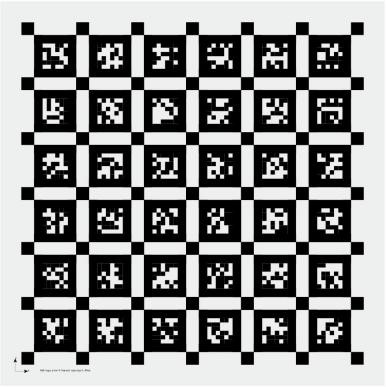
\includegraphics[height=6cm]{figures/april_board}
        \captionof{figure}{April Board上的二维码和棋盘格图案}
        \label{fig:april_board}
    \end{minipage}%
    \begin{minipage}{0.5\textwidth}
        \centering
        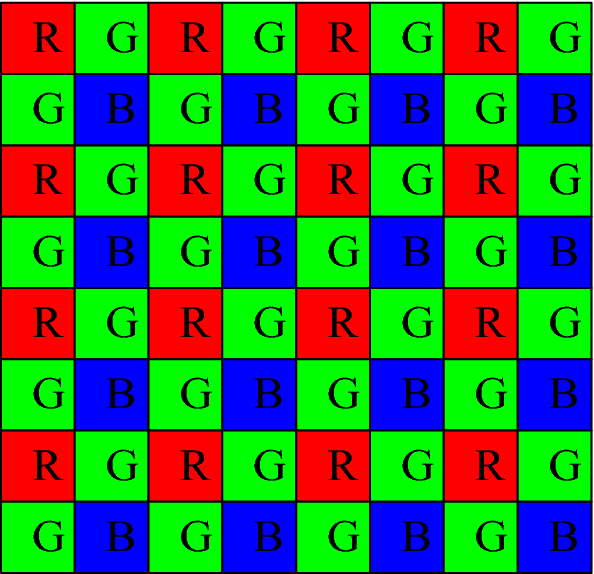
\includegraphics[height=6cm]{figures/bayer}
        \captionof{figure}{Bayer格式照片示意图}
        \label{fig:bayer}
    \end{minipage}%
\end{figure}

本方案中使用的标定物体为April Board,即印有二维码和棋盘格组成的图案的标定板,如图\ref{fig:april_board}所示。
该标定板的尺寸为$800 \times 800$毫米,每个二维码的边长为$88$毫米。
该图案中棋盘格的十字角点可由算法精确完成亚像素级定位,而密集的二维码则便于在不同照片中便捷地匹配角点。
其采用了玻璃基板,以保证标定板的刚性和平整度;
同时采用了氧化铝表面,使标定板表面无明显镜面反射光斑,确保标定板在不同光照条件下的可靠性。

在拍摄标定物体时,需要注意保持相机处于手动对焦模式,关闭光学防抖,以防止其内外参意外发生变化。
并使用前述(第\ref{sec:passive_sync}节)被动相机同步装置同时触发所有相机进行拍摄。转动标定板,重复触发快门15-20次。

\paragraph{相机标定优化目标}
\def\cornerpix{\mathbf{o}}
\def\cornerboard{\mathbf{w}}
本方案中的相机标定算法接收照片中的特征点坐标作为输入,求解上述相机模型中的参数$\camparam$。
正式地,假设共触发了$M$次快门,标定板中共有$K=144$个角点,算法的输入包括第$i$个相机在第$j$次触发快门时拍摄的第$k$个角点($j = 1,2,\cdots,M$、$k = 1,2,\cdots,K$)在像素坐标系中的坐标$\cornerpix_{i,j,k}\in \mathbb{R}^2$;
以及角点在标定板坐标系中的坐标$\cornerboard_k\in \mathbb{R}^3$。
由于每次触发快门时标定板都由人工转动,因此其在世界坐标系中的位置也是未知的,故将第$j$次快门时标定板坐标系到世界坐标系的刚体变换$T_{j}(\cdot)\in \mathrm{SE(3)}$也做为未知量。
其中固定$T_{1}$为幺元,即$T_{1}(X) = X$,以确定世界坐标系的位置。
则本文中的相机标定问题可以表示为以下最小二乘优化问题:
\begin{equation}
    \label{eq:calib_opt}
    \argmin_{\camparam,T} \sum_{i,j,k} \left\| \cornerpix_{i,j,k} - \pi\left(\camparam_i, T_j(\cornerboard_k)\right) \right\|_2^2
    \text{。}
\end{equation}
为实现该目标,首先需要在每张照片中识别角点,并以亚像素级精度精确定位其坐标$\cornerpix_{i,j,k}$。
本节后续将介绍角点的识别、精确定位,模型初始化及上述优化问题的具体求解方法。

\paragraph{角点识别}为识别标定板中可供拟合的角点,本文首先识别照片中的二维码,并将二维码的四个角作为角点的候选点。
本文所用标定板上的二维码为AprilTag,本文实现的识别算法也是基于其开源的方法\cite{AprilTag}。
该算法是一个自下而上的算法,它首先从照片中识别直线段,然后将直线段组合成四边形,最后试图将四边形区域识别为二维码。得益于二维码的纠错功能,虽然该方法召回率稍低,但查准率非常高。同时二维码中存储的信息可用于角点在不同照片中的匹配。

本文所实现的版本的输入为相机拍摄的,原始Bayer格式的照片,该照片是单通道图像,其中RGB像素排列如图\ref{fig:bayer}所示,每$2\times 2$个像素中包括一个红色像素、两个绿色像素和一个蓝色像素。每种像素的传感器前带有滤光片,仅允许特定波长的光被传感器捕获。因此,Bayer格式的照片中,每个像素的值即为该像素对应的颜色通道的光照强度。
为了减少冗余的数据处理流程,并保持全流程的可解释性以准确控制误差,本方案直接使用了原始照片,而没有使用常见的相机后处理后输出的RGB格式图像。

由于我们所拍摄的照片分辨率远超二维码识别所需,因此本文先对照片进行降采样。
其具体方法是,首先在每4个像素中仅取一个绿色像素,以排除颜色对二维码识别的影响;
再进行5倍平均池化,即最终降采样后的图像长宽为原图的$1/10$。
以此降低算法耗时并大大降低照片中的噪声等级,提升算法的鲁棒性。
在低分辨率的图像上完成二维码识别后,二维码的四个角的坐标将被重新映射回完整分辨率的像素坐标,以初始化后续的精确定位步骤。

% 本文使用的相机拍摄的原始照片分辨率高,可达$5472\times 3648$;
% 且宽容度高,其量化后的亮度可达约13000级,相比普通JPG照片仅有256级。
% 因此,本文在\cite{AprilTag}的基础上,设计了尺度、亮度无关的直线段识别算法,使其更加鲁棒,并减少算法超参数调节的麻烦。
% \TODO{尺度、亮度无关的直线段识别算法}

\paragraph{角点精确定位}在上一步识别出角点后,该步骤依据角点周围的像素值,获取这些角点尽可能精确的像素坐标$\cornerpix_{i,j,k}$,以保证标定的精度。
该步骤的难点在于,算法需要对失焦造成的模糊、成像过程中的噪声等因素足够鲁棒,并达到亚像素级的精度。
本文采用的算法为\citet{ROCHADE}提出的精确角点定位算法,其基本思想为:
使用一个二维多项式函数对角点周围的像素进行拟合,然后以该多项式函数的鞍点作为该角点的精确像素坐标。

具体地,本文首先需要从照片原始数据获取单通道灰度图。
该灰度图在标定板区域的每个像素值应表征标定板表面反射的总光强,而不与颜色有关。
为此,需要对红色、蓝色像素值进行缩放,使其与绿色像素匹配(相当于相机的白平衡操作),其缩放系数与环境光照、标定板材质等有关。
本文假设标定板任意位置反射的光线的波长分布是均匀的。
因此,本文首先对上一步求得的二维码区域求凸包,以定位照片中的标定板,并调整缩放系数以使该区域中不同颜色像素的均值相等。
然后,对该图使用半径为$r$的圆锥形kernel进行滤波,以使像素值平滑,从而能更好地被多项式函数拟合。
最后,以角点的当前估计位置为中心,使用二阶二维多项式函数对周围的$2r+1 \times 2r+1$个像素进行最小二乘拟合:
\begin{equation}
    \label{eq:poly}
    \hat{a} = \argmin_{a} \sum_{x,y} \left(\bar{I}(x, y) - (a_0 x^2 + a_1 y^2 + a_2 xy + a_3 x + a_4 y + a_5)\right)^2\text{。}
\end{equation}
在实现上,本方案直接使用解析公式求解该线性最小二乘问题。并求该二维多项式函数的鞍点作为该角点新的估计位置:
\begin{equation}
    \label{eq:subpixel}
    \begin{cases}
        x' &= -\dfrac{\hat{a}_2 \hat{a}_4 - 2 \hat{a}_1 \hat{a}_3}{\Delta} \\
        y' &= -\dfrac{\hat{a}_2 \hat{a}_3 - 2 \hat{a}_0 \hat{a}_4}{\Delta}
    \end{cases},\quad
    \Delta = 4 \hat{a}_0 \hat{a}_1 - \hat{a}_2^2
    \text{,}
\end{equation}
并如此迭代,直到角点的估计位置收敛,该收敛的位置即为$\cornerpix$。
在此过程中,若估计位置超出了图像范围,或$\Delta < 0$,则将该角点排除。
$\Delta < 0$的原因通常是该角点被其他物体遮挡,或者受到其他物体投下的阴影影响。

\def\cornerincode{\hat{\cornerpix}}
在该算法中,$r$的选取可能对结果产生较大影响。较大的$r$将能利用照片中更多像素的信息,从而对噪声更加鲁棒,但也不能过大,否则周边的二维码,或相邻的其他角点等无关信息将影响拟合结果。为此,本文依据上一步识别到的二维码的尺寸以自适应地选择$r$。令$\cornerincode_{i,j}$为照片中第$i$个二维码的第$j$个角点的估计位置,$j\in\{0,1,2,3\}$,以顺时针方向排列,则$r$的选取为:
\begin{equation}
    \label{eq:r}
    \begin{aligned}
        l_{i,\textrm{edge}} & = \min_j\left(\|\cornerincode_{i,j} - \cornerincode_{i,j+1\bmod 4}\|\right)\text{,} \\
        l_{i,\textrm{diag}} & = \min\left(\|\cornerincode_{i,0} - \cornerincode_{i,2}\|, \|\cornerincode_{i,1} - \cornerincode_{i,3}\|\right)\text{,} \\
        r & = \min_i\left\{0.07 l_{i,\textrm{edge}}, 0.05 l_{i,\textrm{diag}}\right\}\text{。}
    \end{aligned}
\end{equation}

\paragraph{多相机内参标定与外参传递}
在第一阶段,本文将对每台相机分别进行标定,获得各相机的内参初始化值
并估计标定版在每次触发快门时与各台相机的相对位置。
具体地,本文依据相机和镜头厂商提供的传感器尺寸、图像分辨率、镜头焦距初始化相机内参$f$、$c$。
然后调用OpenCV中单台相机标定的算法,使用PnP算法求解标定板在每次触发快门时与相机的相对位置$T_{i,j}$;
并使用Levenberg-Marquardt算法对这些参数进行调整。

由于不同相机的同一次快门的触发是严格同步的,因此可以认为若不同相机在同一次快门的触发时,拍摄到的标定板在世界坐标系中的位置是相同的。
据此可将每台相机,以及每次快门触发作为节点,构建二部图,图中的边表示该相机在该次快门中拍摄到了标定板。
若该二部图是连通图,则可迭代地将所有相机、所有快门触发中的标定板的位置传递到世界坐标系中,
如算法\ref{alg:calib_init}所示。
并最终获得$\delta$和$T$中所有参数的初始化值。

\begin{algorithm}[t]
    \caption{外参传递}
    \label{alg:calib_init}
    \begin{algorithmic}[1]
        \Require 连通二部图$(V,E)$;第$j$次快门时标定版坐标系到相机$i$坐标系的刚体变换$\hat{T}_{i,j}\in SE(3),(i,j)\in E$
        \Procedure{外参传递}{$V,E,\hat{T}_{i,j}$}
            \State $C \gets \emptyset$\Comment{已传递的相机集合}
            \State $T_{1} \gets \mathbf{I}$\Comment{以第$1$次快门时标定版坐标系作为世界坐标系}
            \State $S \gets \{1\}$\Comment{已传递的快门触发集合}

            \While{$C \cup S \neq V$}
                \State $i \gets \forall i\in V| i\notin C, \exists j\in S| (i,j)\in E$
                    \Comment{选择与已知位置的标定板相邻的相机}
                \State $U_{i} \gets T_{j}\hat{T}_{i,j}^{-1}$
                    \Comment{相机$i$到世界坐标系的变换}
                \State $C \gets C \cup \{i\}$
                \ForAll{$j | (i,j)\in E, j\notin S$}
                    \State $T_{j} \gets U_{i}\hat{T}_{i,j}$
                        \Comment{第$j$次快门时标定版到世界坐标系的变换}
                \EndFor
                \State $S \gets S \cup \{j\in V| (i,j)\in E\}$
            \EndWhile
            \State \Return $U, T$
        \EndProcedure
    \end{algorithmic}
\end{algorithm}

\paragraph{集束调整}在第二阶段,本文将对所有相机进行集束调整,即直接使用公式\eqref{eq:calib_opt}中的目标函数,在上一阶段的初始化值的基础上,同时优化模型中的所有参数。
具体地,本文使用了Levenberg-Marquardt算法\cite{lm},对目标函数进行优化求解。
并手动实现了公式\eqref{eq:calib_opt}的雅克比矩阵的解析求解算法,以提升算法的速度和收敛精度。

然后,排除掉误差较大的角点,再次重复上述优化过程,并如此迭代数次,每次使用更严格的误差阈值进行排除。
这些误差较大的角点通常是由于角点定位不准确造成的,因此,将其排除后可以提高标定的精度。
该优化过程最终得到的相机参数$\camparam$即为所求的最终的相机标定结果。


\subsection{基于反射球的光源标定和HDRI合成}
\label{sec:light_calib}

除了相机外,在实验室中拍摄,环境光照信息也可以提前采集,从而获得比用算法从人脸照片中估计更精准的结果。
这些信息可用于后续逆渲染的优化之中。
如前文所述,本装置使用的照明为4盏带有柔光箱的摄影灯,均布置在被拍摄对象正面180°的范围内。光源标定的目的是获取被拍摄对象所处的空间中的每个位置上来自每个方向的光照强度,即光场信息。
但本设备的柔光箱据被拍摄对象约1.5米远,相比来说,人脸的尺度较小。因此为简化计算,本文假设所有光线均来自无限远,即该光场的分布近似于与空间位置无关而只与光线入射方向有关。

光照强度和方向的对应关系可被编码在一张HDRI(High Dynamic Range Image,高动态范围图像)中,该图像中的每个像素点对应一个方向,像素点的颜色值则对应于该方向上的光照强度和频率分布。
其与普通的照片保存格式不同,之所以称之高动态范围,是因为其每个像素点的颜色值通常作为浮点数保存,因此可以同时记录很强和很弱的光照,同时保持较高的精度。
使用该技术编码的光照信息也常被用于计算机图形学领域。

\paragraph{数据采集}
为了收集用于合成HDRI的数据,本文将一个全镜面金属的反射球放置于原被拍摄对象头部的位置,然后通过Wi-Fi控制一台靠近中心的相机,继续固定对焦和光圈设置,改变其快门速度和ISO,以捕获该球不同曝光的照片。
通常拍摄的相邻两张照片亮度相差约一倍,共拍摄约8张照片。
这样操作是因为相机的传感器所能记录的最大光照强度是有限的,超出该限制范围的光照信息无法保存在照片中;
而若只使用更低的曝光,则信噪比的下降将导致最终合成的HDRI中的噪声更多。
使用多种不同的曝光参数拍摄即可同时保留亮部和暗部的细节。
后续步骤将直接使用原始Bayer格式的照片,尽可能保留其中信息,同时获取准确的噪声等级估计。

\paragraph{HDRI合成}
该步骤的目的是将上述拍摄的多张照片中各自最可靠的部分(信噪比高,且未超出传感器量程范围)融合为一张HDRI。
为此,本文设计了一种类似卡尔曼滤波的融合算法。
其基本思想是:将不同照片中的同一像素点的读数视为对同一光照强度的不同测量值,不同曝光参数会带来不同的测量噪声方差。
据此对多个观测值加权平均,得到最可能接近真值的最大似然估计值。

本方案使用的相机的传感器中包含了约50万个完全不接受入射光线的像素,这些像素可用于估计黑场(即完全无入射光线时传感器的读数)和测量噪声的方差。
由于数据量非常充裕,这里对每张照片和每个通道分别进行了估计。
记照片$i$中通道$c\in\{\mathrm{r},\mathrm{g1},\mathrm{g2},\mathrm{b}\}$的黑场为$b_{i,c}$,方差为$\sigma_{i,c}^2$。
然后,根据拍摄参数计算每张照片的近似相对亮度,该值与拍摄的曝光时间和ISO设置成正比。
并将照片据此由暗到亮排序为$\mathcal{I}^{(1)}, \mathcal{I}^{(2)}, \cdots, \mathcal{I}^{(n)}$。
原始照片中记录的传感器读数和实际光照强度呈很好的线性关系,
因此可根据读数在每两张相邻照片间通过最小二乘法计算其准确的相对亮度比例:
\begin{equation}
r_i^* = \argmin_{r_i} \sum_{j|\mathcal{I}^{(i+1)}_j < \xi} \left[r_i (\mathcal{I}^{(i)}_j - b_{i,c}) - (\mathcal{I}^{(i+1)}_j - b_{i+1,c})\right]^2
\text{,}
\end{equation}
其中$\xi$为使用ExifTool读取的“线性上界”(Linearity Upper Margin),$j$为像素索引。
该问题为线性最小二乘,可直接求其解析解。
该比例理论上应与之前从拍摄参数计算的值相同,但实际可能由于相机校准误差或其他原因而有所偏差。
最后根据这些相对值$r_i^*$,令任意照片的亮度系数为$1$,可求得所有照片的亮度系数$e_i$。

在获得了这些参数后,假设观测噪声服从高斯分布,即可依照类似卡尔曼滤波的方式从暗到亮递推地合成HDRI。合成的过程可表示为:
\begin{equation}
\begin{aligned}
    \mathcal{J}^{(1)} &= e_1 \left(\mathcal{I}^{(1)} - b_{1,c}\right),\quad
    \hat{\sigma}_{1,c}^2 = e_1^2 \sigma_{1,c}^2 \\
    \mathcal{J}^{(i)}_j &= \begin{cases}
    \frac{e_i^2 \sigma_{i,c}^2 \mathcal{J}^{(i-1)}_j + \hat{\sigma}_{i-1,c}^2 e_i \left(\mathcal{I}^{(i)}_j - b_{i,c}\right)}{\hat{\sigma}_{i-1,c}^2 + e_i^2 \sigma_{i,c}^2} & \text{if } \mathcal{I}^{(i)}_j < \xi \\
    \mathcal{J}^{(i-1)}_j & \text{otherwise}
    \end{cases}\\
    \hat{\sigma}_{i,c}^2 &= \frac{e_i^2 \hat{\sigma}_{i-1,c}^2 \sigma_{i,c}^2}{\hat{\sigma}_{i-1,c}^2 + e_i^2 \sigma_{i,c}^2}
    \quad (i > 1)\text{,}
\end{aligned}
\end{equation}
其中$\mathcal{J}$为每步合成的照片,$\mathcal{J}^{(n)}$即为最终所需的HDRI。
该递推过程与卡尔曼滤波中的融合新的观测值的过程类似,且可以由贝叶斯公式导出,即通过以$\mathcal{J}^{(i-1)}$为均值的先验分布,融合以$e_i\left(\mathcal{I}^{(i)} - b_{i,c}\right)$为均值的观测,推导以$\mathcal{J}^{(i)}$为均值的后验分布。

该融合过程具有以下理想的性质:
较暗的照片信噪比较高,其由于具有较大的$e_i$而在合成时方差较大,从而权重更低;
照片中超出传感器量程($\geq\xi$)的部分则完全不会影响合成结果;
ISO较高的照片由于噪声方差较大,也能自动在合成中降低权重。
% \pdfcomment{TODO 在照片的方差计算中加入photon noise,这是像素较亮时的主导噪音}

\paragraph{像素重映射}
在上一步我们获得了一张反射球的HDRI照片,这张照片中记录了环境中几乎所有方向的光照信息(除了被球挡住的方向)。
但我们仍然需要一种方法将环境光照的方向映射到该照片中的像素坐标上,以便于在渲染时使用。
该映射取决于诸多因素,如用于拍摄的相机的内外参,球在照片中的位置等。
本方案将结合第\ref{sec:camera_calib}节输出的相机参数,使用一种半自动化的方式完成该映射。
与常见的基于正投影的方法相比,本方案使用了相机标定中输出的准确相机参数计算透视投影,因此理论上可以获得更高的精度,但其解算的复杂度也更高。

\begin{figure}
\centering
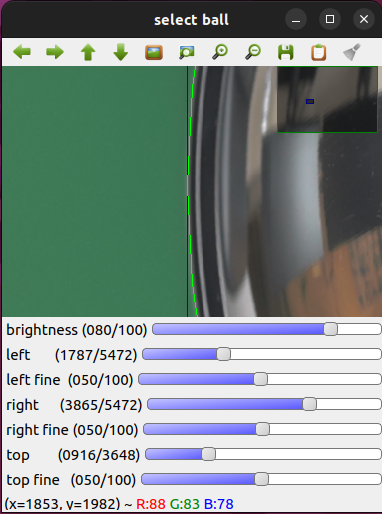
\includegraphics[height=10cm]{figures/sphere_locator}
\caption[反射球位置标注工具界面]{反射球位置标注工具界面。上半部分中蓝色线为当前指定左平面位置,绿色为解算出的反射球位置重投影回像素空间的轮廓}
\label{fig:sphere_locator}
\end{figure}
首先,为了准确得到反射球在照片中的位置,本方案包括了一款标注工具以允许用户手动选中球的位置,如图\ref{fig:sphere_locator}所示。
该工具在上部将显示经过畸变校正的照片,支持自由缩放和平移,以及改变照片的亮度以便观察。在照片上叠加显示了当前选中的球位置的轮廓。
在下部显示了三组滑块,分别用于调整轮廓的左边界、右边界和上边界在照片中的位置。
需要注意的是,这里显示的球的轮廓虽然很接近,但并不是一个圆形。

\def\p{\mathrm}
\begin{wrapfigure}{r}{4cm}
\begin{tikzpicture}
    \filldraw[black] (0,0) circle (2pt) node[anchor=west]{相机$\p{O}$};
    \draw (0,0) -- (0,1.5) node[right=-1mm] {$f_x$} -- (0,2);
    \draw (0,0) -- (-2,2);
    \draw (0,0) -- (2,2);
    \draw [name path=H] (-2,2) -- node[below] {$c_x$} (0,2) -- (2,2);

    \coordinate (C) at (0.3, 3.3);
    \filldraw (C) circle (2pt) node[anchor=west]{$\p{C}$};
    \node[draw, circle] (c) at (C) [minimum size=2.4cm] {};
    \coordinate (A) at (tangent cs:node=c,point={(0,0)},solution=1);
    \coordinate (B) at (tangent cs:node=c,point={(0,0)},solution=2);
    \draw [name path=P1] (0,0) -- ($(0,0)!4cm!(A)$);
    \draw [name path=P2] (0,0) -- ($(0,0)!4cm!(B)$);

    \path [name intersections={of=P1 and H,by=I1}];
    \path [name intersections={of=P2 and H,by=I2}];
    \filldraw (I1) circle (2pt);
    \filldraw (I2) circle (2pt);

    \node [above] at ($(-2,2)!0.5!(I2)$) {$l$};
\end{tikzpicture}
\end{wrapfigure}
在获得了用户输入的左、右、上三个参数后,本文将通过以下算法解算球在相机坐标系下的位置。
首先,由于本文假设光线来自无限远处,因此最终坐标映射的结果将和球的尺度无关,不妨将球的半径设为1。
用户指定的三个参数可各确定一个与球相切的平面,以球心到三个面的距离分别为1的条件联立方程,即可求解出球心的坐标。

右图为整个场景的俯视图,其中下方的三角形代表相机的视锥体,图中标注了相机经过标定后的焦距$f_x$和光心$c_x$。上方的圆代表反射球,两条切线分别表示由用户输入确定的左,右两个平面。
下面以左平面为例,根据用户输入的像素坐标$l$求解左平面的法向量$\mathbf{n}_l$。
在相机坐标系中,取点$\p{A} = (l-c_x, 1, f_x)$、$\p{B} = (l-c_x, 0, f_x)$。
可以验证该两点均投影在像素横坐标为$l$的位置(图中左侧实心点处),
于是可以通过点$\p{O}$、$\p{A}$、$\p{B}$确定该平面,其法向量为
\begin{equation}
\mathbf{n}_l = \overrightarrow{\p{O}\p{A}} \times \overrightarrow{\p{O}\p{B}}
= \left[f_x, 0, c_x - l\right]
\text{。}
\end{equation}
同理可以求得右平面和上平面的法向量$\mathbf{n}_r$、$\mathbf{n}_u$。
记球心坐标为$\p{C}$。
球心到左平面的距离为1可表示为:
\begin{equation}
    \frac {\overrightarrow{\p{O}\p{C}} \cdot \mathbf{n}_l}{\|\mathbf{n}_l\|} = 1
    \text{。}
\end{equation}
对于另外两个平面同理可列方程。
解该线性方程组即可得到球心$\p{C}$的坐标。

在解算出反射球的具体位置后,需要将其重新投影到照片上并绘制出轮廓,以便用户得到实时的反馈。
为此,本方案进一步求该轮廓的参数方程以便绘制。
令曲线参数方程的参数为$\theta\in[0, 2\pi]$。
设球面上一点$\p{D}$,$\overrightarrow{\p{O}\p{D}} = \overrightarrow{\p{O}\p{C}} + [\cos\theta \cos\phi, \sin\theta \cos\phi, \sin\phi]$,其中$\phi$为未知数。
令$\overrightarrow{\p{O}\p{D}}$与球面相切,可由$\overrightarrow{\p{O}\p{D}} \perp \overrightarrow{\p{C}\p{D}}$列方程求解$\phi$:
\begin{equation}
\begin{aligned}
&\overrightarrow{\p{O}\p{C}} \cdot \overrightarrow{\p{C}\p{D}} = -1 \\
\Rightarrow &a \cos\phi + \p{C}_z \sin\phi = -1, \quad a = \p{C}_x * \cos(\theta) + \p{C}_y * \sin(\theta)\\
\Rightarrow &\phi = \arcsin\frac{-1}{\sqrt{a^2 + \p{C}_z^2}} - \arctan\frac{a}{\p{C}_z^2}
\text{,}
\end{aligned}
\end{equation}
其中最后一步推导使用了辅助角公式。然后点$\p{D}$在像素坐标系中的投影即为所求的反射球的轮廓曲线上的一点,其关于$\theta$的参数方程可用于便捷地绘制出该轮廓。

最后,利用反射球的位置,我们需要解算光照方向与像素坐标的映射关系。
对于像素坐标上的一点$e$,可将其映射为相机坐标系中的一条源自原点射线,其方向为:
\begin{equation}
    \mathbf{v} = \left[\frac{e_x-c_x}{f_x}, \frac{e_y-c_y}{f_y}, 1\right]
    \text{,}
    \label{eq:ray1}
\end{equation}
该方向是视线方向,也即光线从反射球反射的相反方向。
该射线与反射球表面交于一点$\p{E}=\lambda\mathbf{v}$,且满足:
\begin{equation}
    \left\| \overrightarrow{\p{O}\p{E}} - \overrightarrow{\p{O}\p{C}} \right\| = 1
    \text{。}
    \label{eq:ray2}
\end{equation}
在$\mathbf{E}$处,球面的单位法向量为$\mathbf{n}=\overrightarrow{\p{O}\p{E}}$,视线反射的方向为$\mathbf{r}$。
根据光线反射的原理,$\mathbf{r}$、$\mathbf{v}$、$\mathbf{n}$位于同一平面且入射角等于出射角,有:
\begin{equation}
    \mathbf{r} = \mathbf{v} - 2(\mathbf{v} \cdot \mathbf{n}) \mathbf{n}
    \text{。}
    \label{eq:ray3}
\end{equation}
联立公式\eqref{eq:ray1}至\eqref{eq:ray3}即可获得所求像素坐标$e$与光照方向$\mathbf{r}$的映射关系。
理想中应当对给定的任意$\mathbf{r}$求解其所对应的像素坐标$e$,
但方程组的求解过于复杂,因此本方案选择从像素坐标$e$出发,对每个像素求解其对应的光照方向$\mathbf{r}$。
在使用时,对于任意给定的$\mathbf{r}$,从与其最相近的3个准确对应了某个像素的方向中插值,从而近似地获取其对应的像素坐标$e$。

为了得到可直接在下游任务中使用的环境光照贴图,本方案利用了OpenGL实现上述插值过程。
具体来说,本方案为照片中反射球所在区域的每个像素处生成一个顶点,并连接相邻像素形成三角形网格。
然后以上一步合成的反射球HDRI照片作为纹理贴图,从像素坐标计算每个顶点的纹理坐标,并按照计算的$\mathbf{r}$将其放置在3D单位球上的对应位置。
最后使用OpenGL光栅化渲染所生成的网格,在片元着色器中根据纹理坐标对HDRI采样和插值。
根据所需环境光照贴图的格式不同,可使用不同的顶点着色器完成对应的顶点坐标变换。
本方案中已支持常见的等距柱状投影(Blender中使用)和立方体贴图(nvdiffrast中使用)两种格式。

\subsection{主动相机/闪光灯同步}

上述软硬件方案已能支撑被动光源采集的整个流程。
但本方案还希望能加入对主动光源的支持,以便能实验和对比不同重建方法的优劣。
然而,本方案所使用的消费级相机带来了很大的限制:这些相机在照片模式下无法在很短时间内连续拍摄多张照片,而在视频模式下又缺少不同相机间精确同步的方法。
所以本文主要参考了\citet{FyffeGTGD16}的方案,使用多盏闪光灯依次以数毫秒的间隔闪光,并将相机分为多组,每组同步到不同的闪光灯上,
以达成同时捕获不同视角和不同光照的照片的目的,为重建提供更多信息。

为了完成对闪光灯和相机的控制,本方案设计了一个主动相机同步装置。
它带有一个单片机以完成可定制的实时控制,能独立控制每台相机、闪光灯触发延迟,最多可控制24台设备。
以下部分将进一步介绍该装置的设计和使用。

\paragraph{主动同步装置硬件设计}

\begin{figure}
\centering
\begin{tikzpicture}[
    node distance=0.2cm,
    part/.style={rectangle, draw=black, minimum width=4cm, minimum height=1cm, align=center},
    conn/.style={above, font=\small},
    inner/.style={part, fill=black!10},
    io/.style={part}
]
    \linespread{1.2}
    \node (sync_in) [io]{外部同步接口};
    \node (btn_in) [io, below=of sync_in]{4路按钮输入};
    \node (shift_out) [inner, below=of btn_in]{移位寄存器};
    \node (sync_out) [io, right=of shift_out]{24路相机/闪光灯同步接口};
    \node (oled) [io, below=of shift_out]{OLED显示模块};

    \node (stm32) [
        inner,
        minimum width=0,
        minimum height=4.6cm,
        left=1.2cm of $(btn_in.west)!0.5!(shift_out.west)$
    ]{STM32\\最小系统};
    \node [
        inner,
        minimum width=0,
        minimum height=0,
        above=of stm32.south,
        fill=brown!20
    ]{3.3V\\供电};

    \draw [<-] (stm32.east |- sync_in)   -- node[conn]{GPIO} (sync_in);
    \draw [<-] (stm32.east |- btn_in)    -- node[conn]{GPIO} (btn_in);
    \draw [->] (stm32.east |- shift_out) -- node[conn]{GPIO} (shift_out);
    \draw [->] (stm32.east |- oled)      -- node[conn]{I2C}  (oled);

    \draw [->] ($(stm32.west) - (1.5cm, 0)$) -- node[conn]{USB} node[conn,below]{5V电源} (stm32);
\end{tikzpicture}
\caption{主动同步控制器硬件拓扑结构}
\label{fig:active_sync}
\end{figure}
图\ref{fig:active_sync}展示了本方案中设计的主动同步控制器的硬件拓扑结构。
该装置以一块STM32F103C8T6单片机为核心。
它通过GPIO接口,控制3块串联的74HC595D 8位移位寄存器,以控制最多24台相机或闪光灯。
作为系统指令输入和状态的反馈,该装置通过GPIO连接有4个机械按钮,可由软件指定其具体功能,并通过I2C总线连接了一个OLED显示屏模块。
此外,为了提升装置的可扩展性,还预留了一个用于外部同步的接口,可接收来自外部的对焦和快门触发同步信号,也连接到了单片机的GPIO接口。

\paragraph{主动同步控制器固件设计}
为驱动控制器中的单片机,需要为其编写固件。该装置的固件设计有如下几个总体目标:
\begin{enumerate}
\item 高精度:使每个设备触发的时间点尽可能接近设置的时间点。
\item 离线配置:每个设备的触发时间都能直接在触发装置上调节,而不需要连接电脑。这允许在实验时快速调整配置。
\item 节能:考虑到可能需要使用电池供电,本装置应尽可能节约能量,以避免不必要的电池充电或电缆拔插。
\end{enumerate}
后文(第\ref{sec:sync_impl}节)将介绍其具体实现。

虽然相机和闪光灯的触发原理相似,但是它们响应触发信号的速度是不同的,因此需要在设定的触发时序中为闪光灯加入一定的延迟。
下文将介绍一种利用滚动快门实现的该延迟标定的方法。

\begin{wrapfigure}{r}{4.7cm}
    \begin{tikzpicture}
        \zihao{5}
        \draw[->] (0,0) -- (0,3) node[right] {感光元件行};
        \draw[->] (-0.2,0) -- (4,0) node[below] {时间};
        \def\s{0.5}
        \def\sp{1.0}
        \def\dur{1.7}
        \def\h{2.2}
        \filldraw [fill=blue!30,draw=none] (\s,\h) -- (\s+\sp,0) -- node [below] {曝光时间} (\s+\sp+\dur,0) -- (\s+\dur,\h);
        \filldraw [fill=blue!50,draw=none] (\s+\sp,\h) -- (\s+\sp,0) -- (\s+\dur,0) -- (\s+\dur,\h);
        \draw (\s,\h) -- (\s+\sp,0) -- (\s+\sp+\dur,0) -- (\s+\dur,\h);
        \draw (0,\h) -- (\s+\dur,\h);
        \draw [thin,draw=blue!50] (\s+\sp,0) -- (\s+\sp,-0.5);
        \draw [thin,draw=blue!50] (\s+\sp+\dur,0) -- (\s+\sp+\dur,-0.5);

        \def\flash{1.2}
        \draw (\flash,2.5) -- (\flash,-1) node [right] {闪光灯触发};
    \end{tikzpicture}
    \caption{滚动快门原理}
    \label{fig:rolling_shutter}
\end{wrapfigure}

\paragraph{滚动快门原理}
本方案使用的相机快门模式是电子前帘快门,其工作方式是首先由电路依次给感光元件的每一行像素通电,使其开始接收光线。
然后由一块塑料板(快门)快速落下,以同样的顺序依次挡住每一行像素,使其停止接收光线。
如右图\ref{fig:rolling_shutter}所示,每一行像素接收光线的时间即为相机中设定的曝光时间。
但每一行像素的曝光并不是在同一时刻,且这个延迟,即右图中的斜率是无法调节的,它受限于快门下落的速度。

相对来说,闪光灯闪光的时间非常短。
因此,若要使用闪光灯拍摄正确曝光的照片,则需要将曝光时间设置得足够长,以保证至少在某一时刻所有像素在同时接收光线,且需要将闪光灯触发的时刻设置到这段同时接收光线的时间(右图中深色填充区域)。
如右图\ref{fig:rolling_shutter}标注的闪光灯触发时间点则只能得到上半亮下半暗的照片。

\paragraph{闪光灯触发延迟快速标定方法}
为了获取准确的闪光灯触发延迟,利用上述原理,本文设计了一种快速标定流程:
\begin{enumerate}
\item 将相机快门速度设置到1/2秒。
\item 通过二分搜索,找到一个触发延迟,使拍摄照片上半亮下半暗。
此时闪光灯时间位置在图\ref{fig:rolling_shutter}中标注的位置。
\item 以0.5毫秒为步长,逐步增加延迟,直到拍摄照片全亮。
同时根据调整过程中明暗分界线移动的速度,估计快门滚动所需时间。
\item 调整相机快门速度设置,使其稍大于所估计的快门滚动所需时间。
\end{enumerate}
根据该流程,本项目所使用的相机需要比闪光灯早触发约47毫秒时可正常曝光。
相机的快门速度最终设定为1/200秒。

\subsection{照片拍摄和整理流程}
\label{sec:photo_process}

虽然该方案采用了部分自动化控制的手段,但在采集拍摄的过程中依然需要较多的人工参与。
本节将介绍该方案中的人工操作标准流程,并介绍了一些其他用于辅助减少工作量的小工具。

\paragraph{同步装置连接与设定}
在开始拍摄前,需要将相机、灯光等设备固定到预定位置,并连接同步控制器。
当使用被动同步装置时,可在左右分设两个控制器分别连接附近的相机,再将两个控制器相连。
主动同步装置由于成本较高,目前只有一个,因此需要将所有相机和闪光灯连接至该控制器,并需要较长的线缆。
主动同步装置还需根据设定的拍摄方案和标定的触发延迟进行设定。
连接完成后,需试拍几张以确定软硬件设定是否正确。

\paragraph{拍摄采集对象}
在拍摄前需要根据光源设置和实验目的设置相机的快门,光圈,ISO等参数。
光圈的设置要保证足够的景深,以免失焦模糊丢失过多信息,可设置在F8;
快门速度被动同步时可设置在1/30秒,主动同步时则按照标定的设置;
ISO设定在比相机自动测光低1至2 EV的值,在降低噪声的同时,尽量保证镜面反射的高光区域不超出量程。
然后在预计被采集对象脸部位置上放一个参照物,并使相机自动对焦到该参照物上,再切换到手动对焦模式。
在每一个人采集前,需仔细放大观察相机预览图,并指导被采集者调整姿势,使其脸部处于每台相机的焦点中。该步骤较为繁琐。
调整完成后,通过控制器触发快门4次,以防某次触发快门时出现意外。

\paragraph{相机、光源标定数据采集}
在采集完人脸数据后,需要按照第\ref{sec:camera_calib}节中的方法采集相机标定数据,以及按照第\ref{sec:light_calib}节中的方法采集光源标定数据。
最后再在没有被拍摄物的情况下,采集一组背景照片。

\paragraph{照片拷贝和整理}
在完成所有采集后,需要将所有照片拷贝到计算机上,整理以供后续算法使用。
本文尝试了使用相机内建的Wi-Fi功能进行自动化,但链接速度过于缓慢,最终没有采用。
于是本方案最终使用了半自动化的方式。
如图\ref{fig:copy_photo}所示,
在计算机中运行一个自动拷贝进程,它利用Linux的udev系统监听SD卡连接计算机的事件。
利用该程序,手工从相机中取出SD卡后,只需将卡插入读卡器,程序便会自动完成挂载、拷贝、卸载的过程,之后需在提示时手工拔出并换入下一张卡。全程无需对计算机进行任何操作。
\begin{figure}[htbp]
\centering
\begin{tikzpicture}
    \node [rectangle,draw=black,rounded corners=3mm] (start) {进程启动};
    \node [rectangle,draw=black] (wait) [right=of start] {等待SD卡插入};
    \node [rectangle,draw=black] (mount) [right=of wait] {挂载SD卡};
    \node [rectangle,draw=black] (copy) [right=of mount] {拷贝照片};
    \node [rectangle,draw=black] (unmount) [below=of mount] {卸载SD卡};
    \node (manual) [below=of wait] {手动插入下一张卡};

    \path [->] (start) edge node {} (wait)
        (wait) edge node {} (mount)
        (mount) edge node {} (copy)
        (copy) edge node {} (unmount)
        (unmount) edge node {} (wait)
        (manual) edge node {} (wait);
\end{tikzpicture}
\caption{半自动照片拷贝进程流程图}
\label{fig:copy_photo}
\end{figure}

然后,在计算机中需要人工对大量拍摄的照片进行筛选、分类,以去除不符合标准的照片,并将不同照片送入不同的下游流程处理。
\begin{figure}
\begin{tikzpicture}[]
    \node (ui) [inner sep=0, outer sep=0, anchor=south west] {
        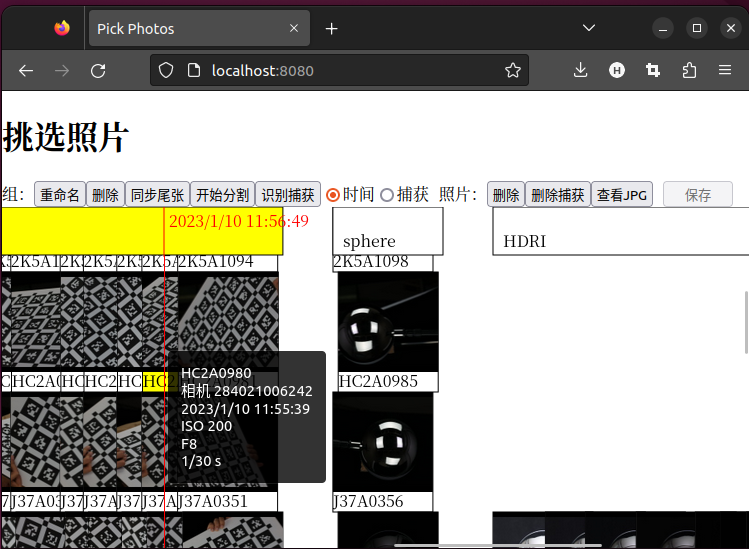
\includegraphics[width=\textwidth,trim={2 0 0 49},clip]{figures/pick_photo}
    };
    \color{blue};
    \node at ( 9.5,4  ) {\textcircled{1}};
    \node at ( 7.5,7  ) {\textcircled{2}};
    \node at ( 6.5,4.4) {\textcircled{3}};
    \node at ( 3.2,7  ) {\textcircled{4}};
    \node at ( 1  ,8.1) {\textcircled{5}};
    \node at ( 2  ,8.1) {\textcircled{6}};
    \node at ( 3  ,8.1) {\textcircled{7}};
    \node at ( 4.3,8.1) {\textcircled{8}};
    \node at ( 5.7,8.1) {\textcircled{9}};
    \node at ( 7.1,8.1) {\textcircled{10}};
    \node at (10.6,8.1) {\textcircled{11}};
    \node at (11.6,8.1) {\textcircled{12}};
    \node at (12.9,8.1) {\textcircled{13}};
    \node at (14.4,8.1) {\textcircled{14}};
\end{tikzpicture}
\caption[照片整理工具UI截图]{照片整理工具UI截图。图中带圈数字是为解释说明而附加的,并非UI中的元素。
界面中横轴为时间轴,每一行为同一台相机拍摄的照片。\\
\textcircled{1}照片预览图和文件名,黄色背景表示选中的照片\\
\textcircled{2}照片组名,黄色背景表示选中的组\\
\textcircled{3}鼠标悬浮提示框,显示照片曝光信息等元数据\\
\textcircled{4}游标,辅助视觉对齐并显示当前鼠标位置表示的时间\\
\textcircled{5}重命名选中照片组\\
\textcircled{6}删除选中照片组\\
\textcircled{7}以选中组最后一张对齐为标准同步不同相机时间戳\\
\textcircled{8}在下一次单击的位置将选中组分为两部分\\
\textcircled{9}运行算法自动匹配选中组中属于同一次捕获的照片\\
\textcircled{10}切换下方横轴显示模式\\
\textcircled{11}删除选中照片\\
\textcircled{12}删除与选中照片同一次捕获的所有照片\\
\textcircled{13}在新窗口查看选中照片的全分辨率JPG预览\\
\textcircled{14}保存当前分组和时间戳同步信息
}
\label{fig:pick_photo}
\end{figure}
为此,本方案中包含了一个基于Web的照片整理工具。其界面如图\ref{fig:pick_photo}所示。
该工具可以快速从CR3格式的照片中提取预览图和高分辨率的预览JPEG图,以便于快速浏览。
该工具可以识别拍摄相机的序列号,将同一台相机的照片放在一行。
并利用照片中记录的时间戳信息,将照片按照时间顺序排列,根据时间间隔自动分组。
然后,用户可根据需要对组进行重命名、删除、拆分等操作。
用户也可以删除单张照片,或单次捕获的所有照片。
此外,本工具还包含了一个基于贪婪算法的捕获匹配程序,用于自动匹配同一次快门捕获的所有不同相机拍摄的照片,并可输入后续的相机标定等算法。
操作完成后,本工具保存的数据格式可直接对接后续标定等软件,也可重新导入本工具,以便于后续的修改。
该工具基于Web技术开发还有一个额外的好处,用户可以在任意终端上完成整理工作,而不需要在本地安装任何软件,也不需要在本地拷贝大量的照片数据。
有关该工具的更多实现细节,可参见附录\ref{app:pick_photo_impl}。

\section{方案实现与验证}

本节将介绍上述方案的具体实现方式,并对该方案所采集到的数据开展了一些验证性的实验。

\subsection{支撑机械结构制造}

本文实现的硬件布局主要是参考了\citet{RiviereGBGB20}所展示的布局。
首批配置了12台相机和4台带有柔光箱的摄影灯,并按前述方案分别固定在相机支架和灯架上。

\begin{figure}
    \centering
    \begin{subfigure}[b]{0.2\textwidth}
        \centering
        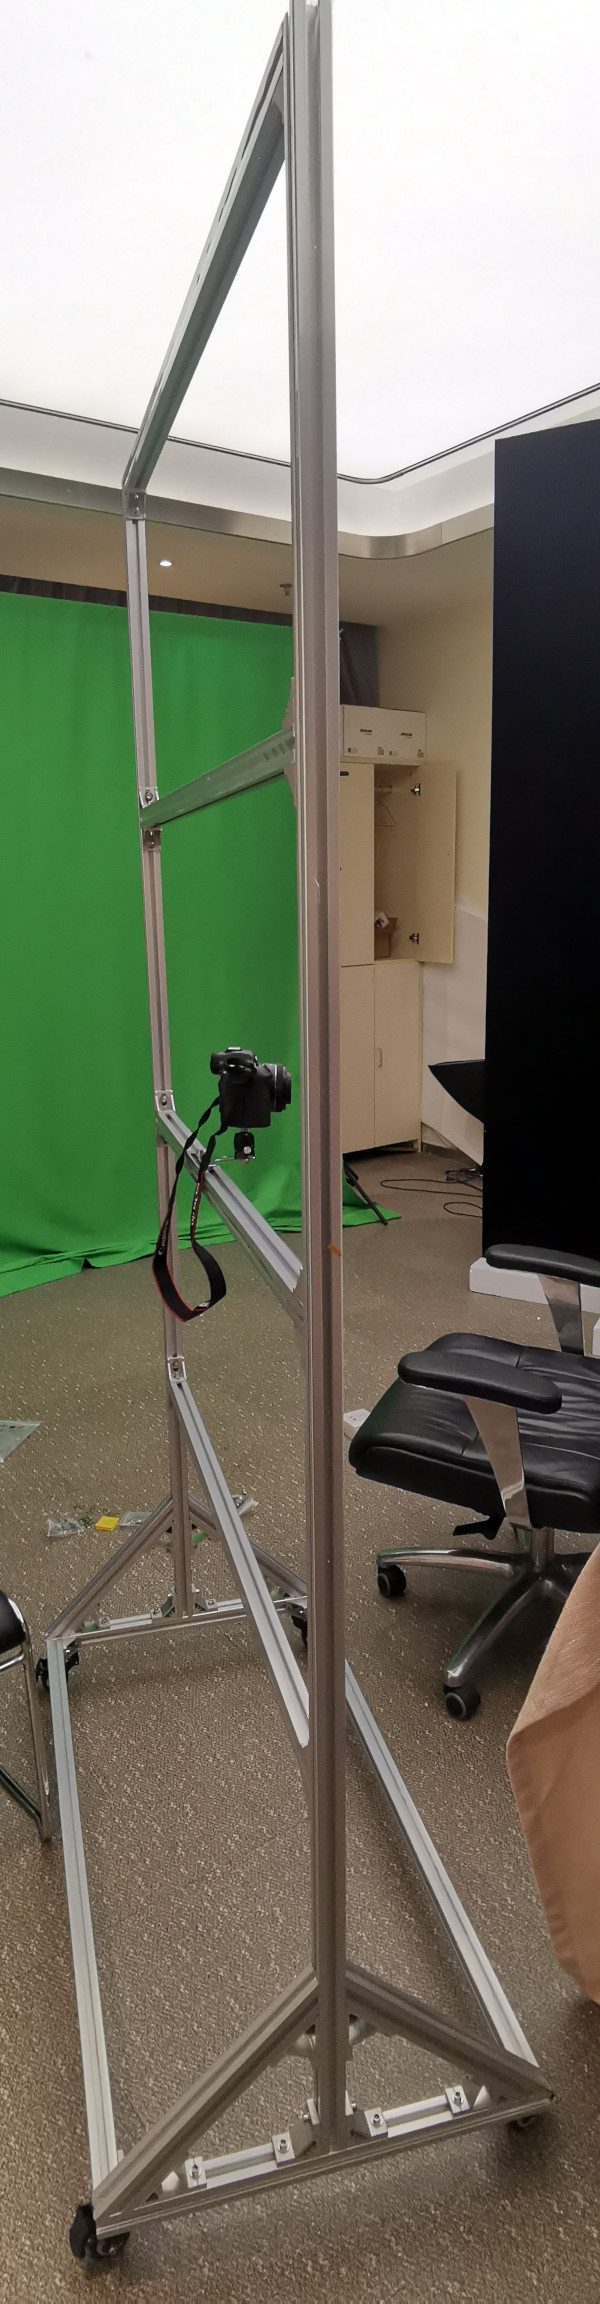
\includegraphics[height=7cm]{figures/frame-impl}
        \caption{组装完成照片}
    \end{subfigure}
    \begin{subfigure}[b]{0.47\textwidth}
        \centering
        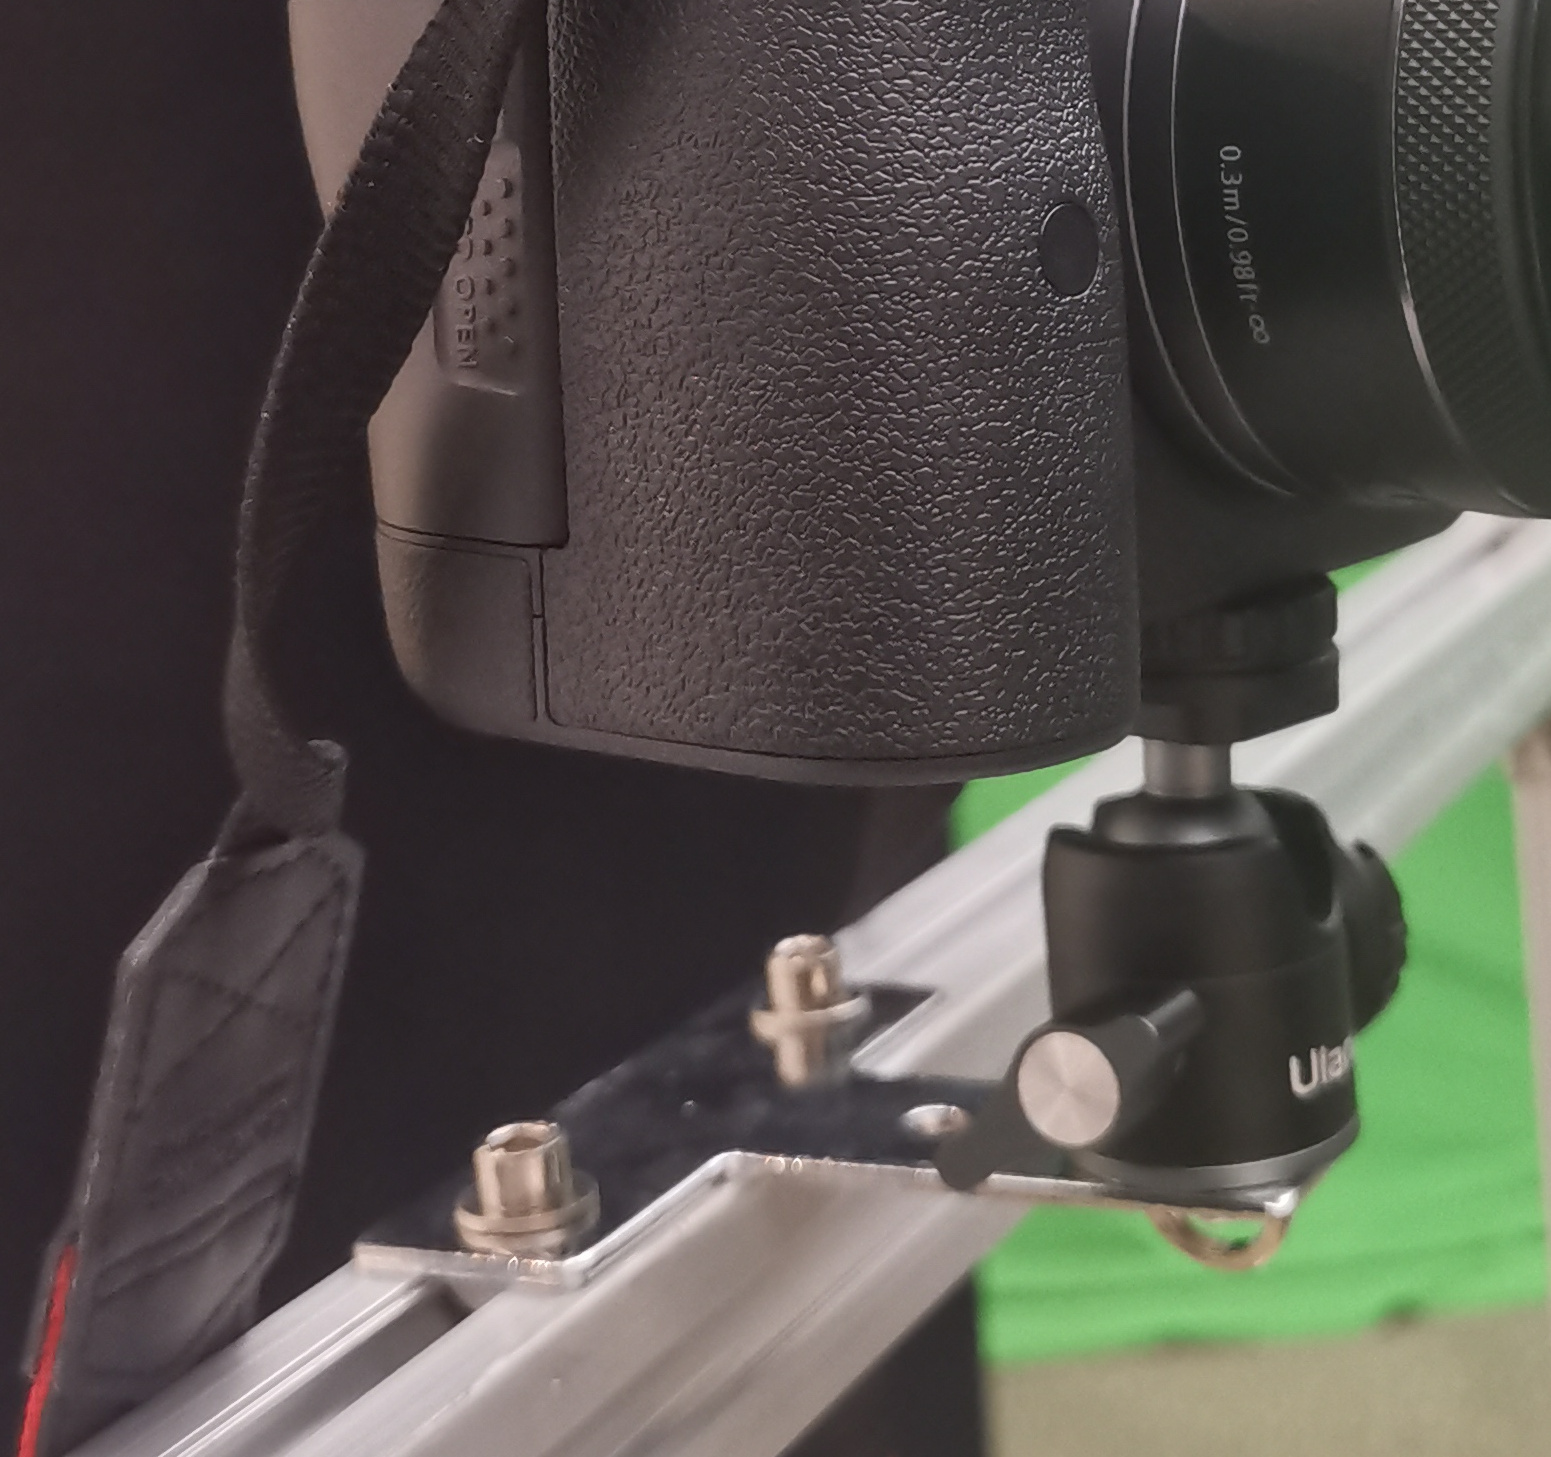
\includegraphics[height=7cm]{figures/frame-camera}
        \caption{相机固定}
    \end{subfigure}
    \caption{铝型材支架的设计和实现}
    \label{fig:frame}
\end{figure}

图\ref{fig:frame}展示了相机支架实现。
单个支架的主体部分由4个2寸脚轮,12.47米3030铝型材以及若干连接件组成。
设计全高2.103米,长1.06米,宽0.53米。
其物料成本约需要700元。
考虑到实验场地可能的变动,支架装配有4个脚轮,方便移动,且这些脚轮带有锁定功能,在使用时也能固定支架的位置。
脚轮固定在矩形底座上,底座则通过大量连接件,尽可能稳固地支撑了两根2米长的竖直铝型材。
在竖杆之间设计有4根长1米的横杆,构成多个高度层,每两根间设计间距为0.5米。
得益于本方案使用T型螺母固定,无需打孔,因此高度层的高度和相机固定的位置均可根据需要随时调整。
为固定相机,本方案首先将T型连接板通过T型螺母固定在铝型材上,然后将一个球形云台通过1/4英寸螺栓固定在连接板上,最后将相机通过标准的1/4英寸接口固定在云台上。

总的来说,该支架支撑稳定,使用灵活,完全满足了固定12台相机的需求,为其他部分的实现打下了良好的基础。

\subsection{相机同步装置实现}
\label{sec:sync_impl}

为实现方案中的相机同步控制器,本文使用了PCB打样服务和一些廉价电子元件。

\paragraph{被动同步控制器}

\begin{figure}
    \centering
    \begin{minipage}{0.49\textwidth}
        \centering
        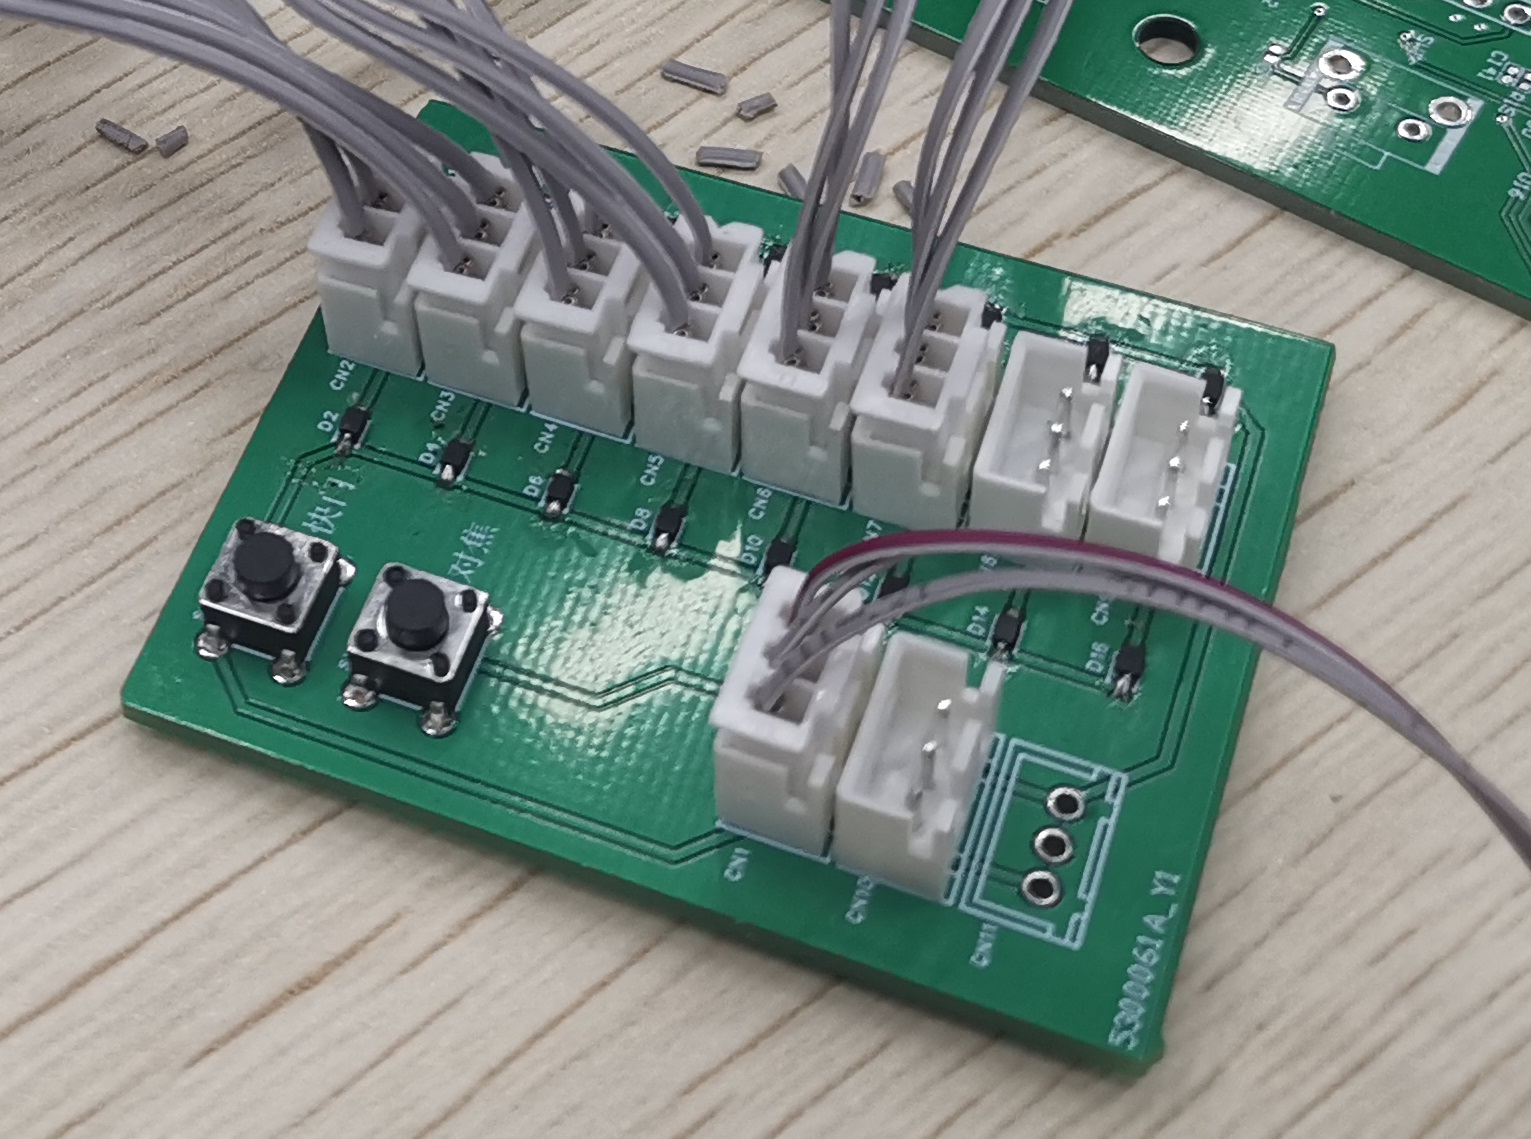
\includegraphics[height=5.8cm]{figures/passive_sync_controller}
        \captionof{figure}{被动同步控制器实物照片}
        \label{fig:passive_sync_photo}
    \end{minipage}\hfill%
    \begin{minipage}{0.5\textwidth}
        \centering
        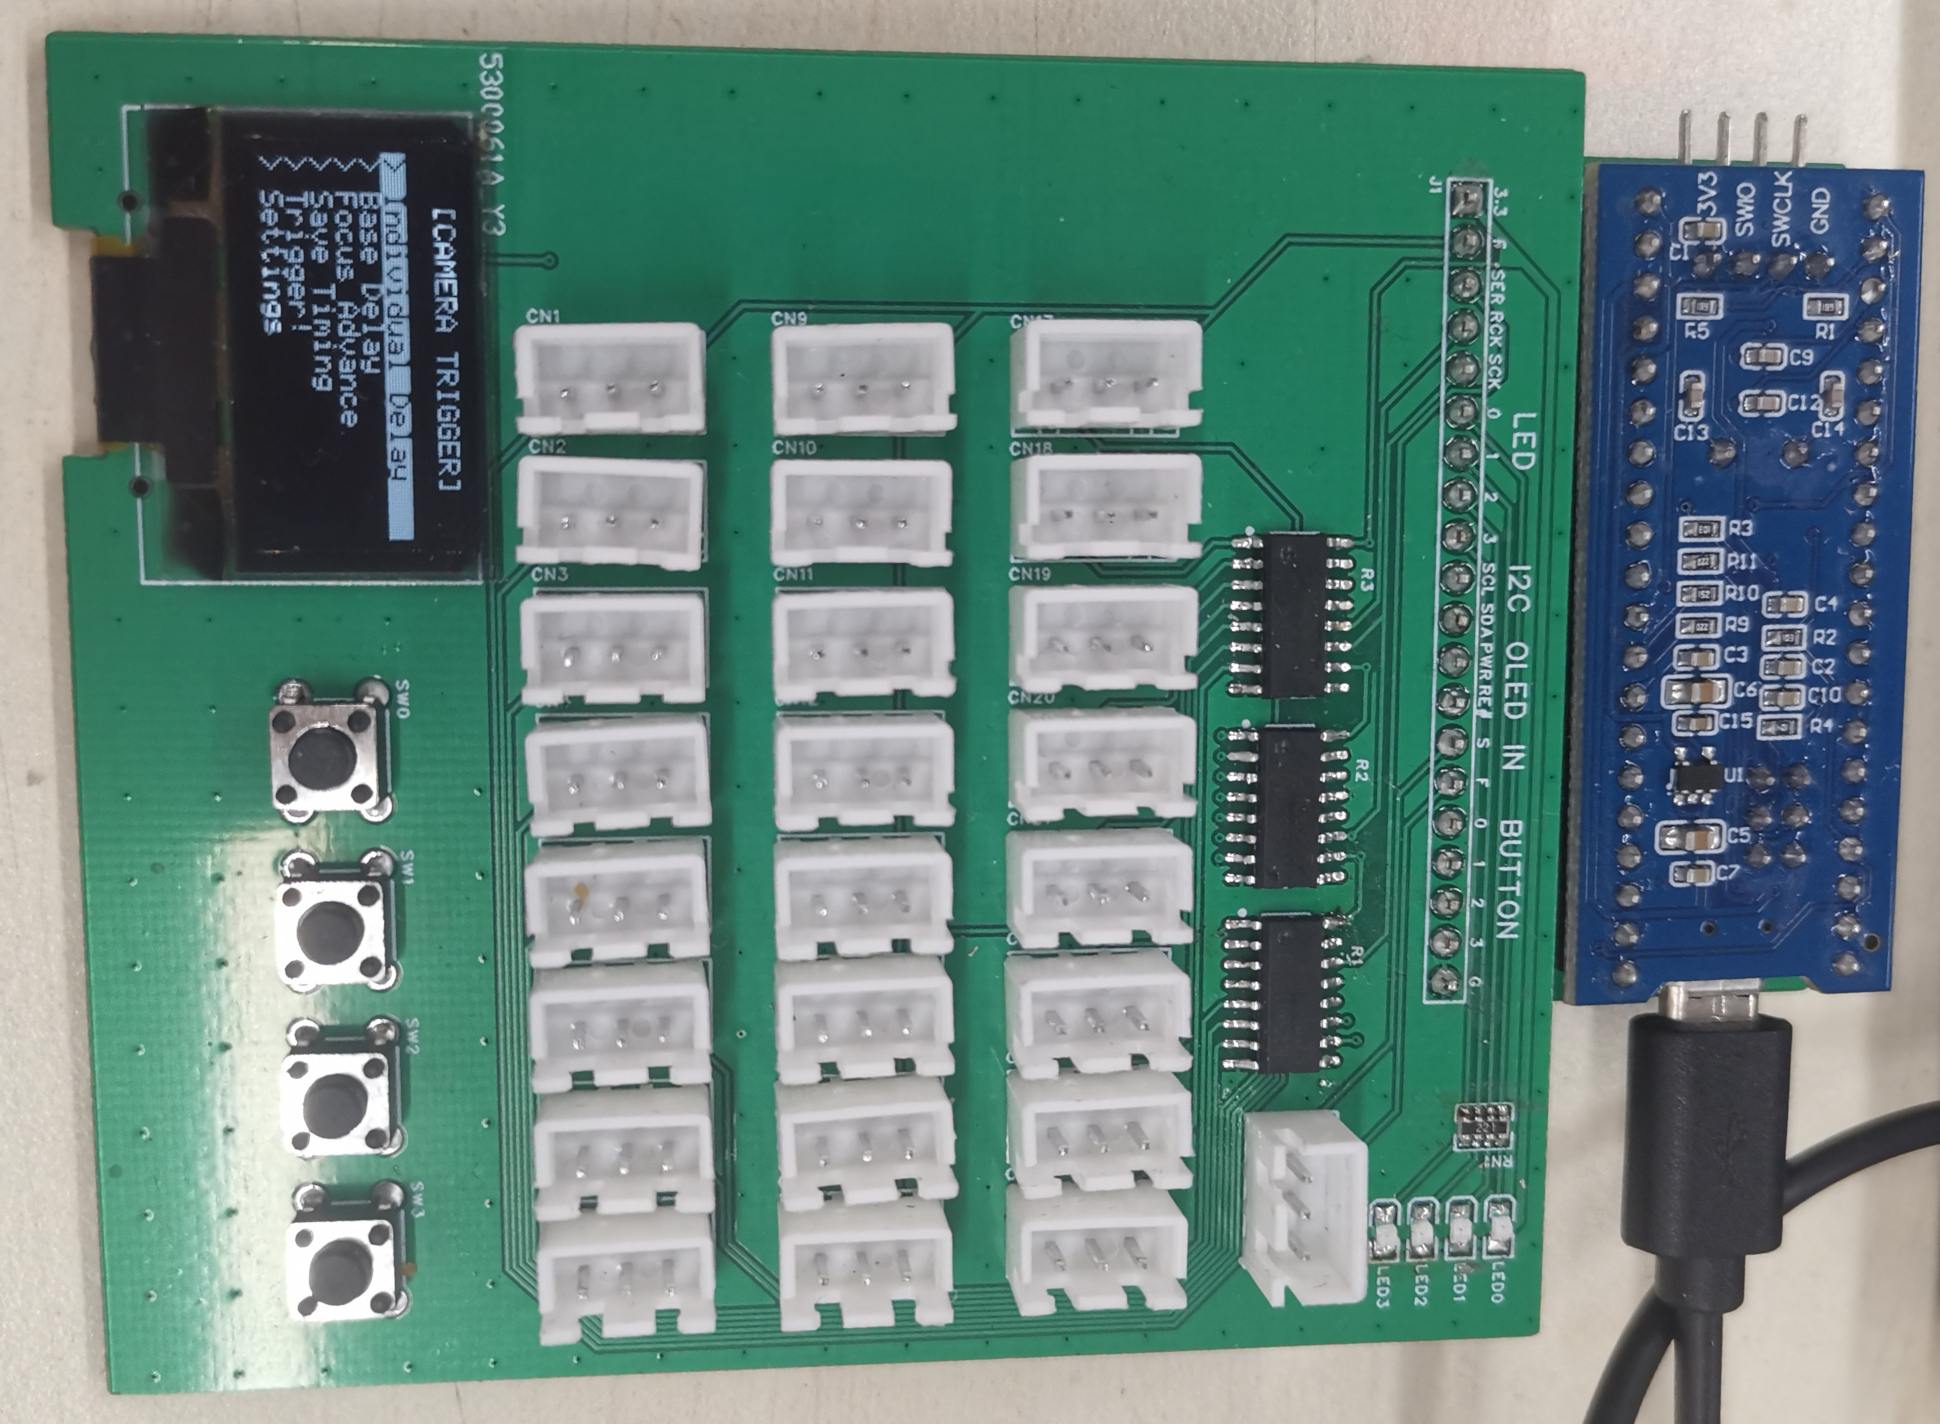
\includegraphics[height=5.8cm]{figures/active_sync_photo.jpg}
        \captionof{figure}{主动同步控制器实物照片}
        \label{fig:active_sync_photo}
    \end{minipage}%
\end{figure}

其中,每个被动同步控制器的照片如图\ref{fig:passive_sync_photo}所示。
控制器无需供电,它用机械按钮短接控制线和地线,从而触发相机快门。
控制器之间,以及相机与控制器间均采用AWG28规格的排线连接,
在控制器端均使用了冷压的XH2.54插头;
在相机端则使用了焊接的2.5mm插头。
此外,每个相机接口在连接到总线前均使用了两颗二极管进行隔离,以防止相机间的干扰。
这样可允许在控制器连接后依然可以手动控制单台相机的快门,也能防止在连接线缆时误触发快门。
更多实现细节可参见附录\ref{app:passive_sync}。

\paragraph{主动同步控制器}
主动同步控制器采用单片机控制外置的移位寄存器以控制相机。
这是为了节省单片机的IO接口,
同时由于移位寄存器能通过单个电信号同时切换所有输出引脚的状态,这种设计也能实现更加精确的触发控制。
所采用的移位寄存器是富满FM生产的,该芯片输出引脚的功能与常见的推挽输出不同,它的输出引脚是开漏模式,
即当输出引脚为高电平时,该引脚呈高阻态,反之为低电平时,该引脚接地。
由于每个相机、闪光灯以及本控制器都是独立供电的,这种设计能起到一定的隔离作用,也能避免不同设备间由于电压不匹配造成的潜在问题。

在硬件实现上,单片机最小系统部分是市面上购买的集成电路,其中包括USB供电,5V转3.3V的电压转换模块,晶振,以及单片机本身。
其余IO接口部分则是定制的PCB板,并通过另一块定制的连接板将其连接到最小系统上。
图\ref{fig:active_sync_photo}展示了该装置组装完成后的实物照片。
与相机的连接线则可以复用被动同步装置中所使用的。
本方案选用的神牛闪光灯的触发方式与相机类似,但它使用的是6.35mm的插头,且无对焦控制线。因此在相机连接线的基础上更换焊接的插头即可。

在固件实现上,
为实现各种配置功能,本程序主体基于事件循环的模式。
在每次循环中处理按钮的IO事件,并刷新OLED的界面显示。
\begin{figure}
\centering
\begin{subfigure}[b]{.41\textwidth}
    \begin{tikzpicture}[
        state/.style={circle, draw, minimum size=1.5cm, inner sep=0pt, align=center},
        initial/.style={state, fill=black!50, text=white},
        every edge/.style={draw, bend left=10pt, ->},
    ]
        \linespread{1}\zihao{5}
        \node (offline) [state, initial] {断电};
        \node (standby) [state, right=of offline, label={below,align=center:16mA\\(主菜单)}] {待机};
        \node (sleep) [state, right=of standby, label=below:2.5mA] {休眠};
        \node (test) [state, above=of standby] {测试\\模式};
        \node (timer) [state, above=of sleep, label=25mA] {高精度\\定时};

        \path (offline) edge (standby)
                        edge node [sloped,above] {按住按钮3} (test)
              (standby) edge (sleep)
                        edge (timer)
              (sleep)   edge (standby)
              (timer)   edge (standby);

    \end{tikzpicture}
    \caption{状态机}
    \label{fig:active_sync_states}
\end{subfigure}%
\begin{subfigure}[b]{.59\textwidth}
    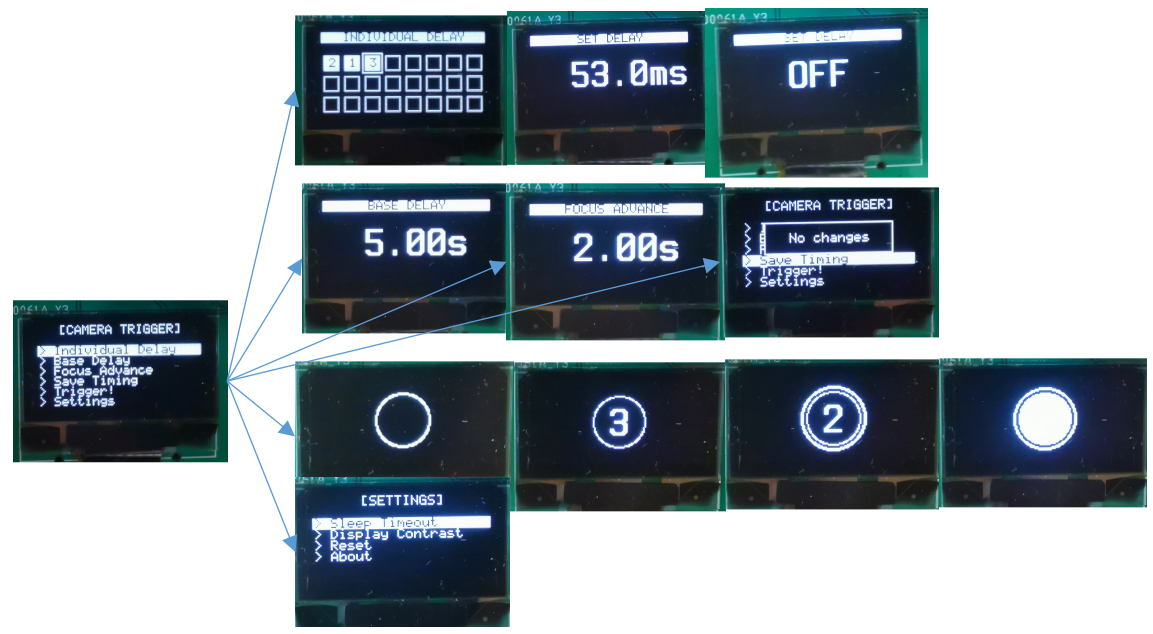
\includegraphics[width=\textwidth]{figures/active_sync_ui}
    \caption{用户界面}
    \label{fig:active_sync_ui}
\end{subfigure}%
\caption{主动同步装置软件设计}
\end{figure}
此外本程序还实现了如图\ref{fig:active_sync_states}所示的简单的状态机以实现上述目标。
按住按钮3的情况下插入电源即可进入测试模式,可用于测试硬件组装是否正常。
上电后进入待机状态,此时可进行各项参数的设置。在各级菜单设置界面,由于并无高实时性需求,单片机将降低主频运行,且在每次事件循环后进入数毫秒的低功耗状态,以节省能量。
同时按钮可以以中断的形式唤醒单片机,所以该策略并不影响用户输入的响应速度。
当一段时间用户没有操作时,将关闭OLED显示屏,并且单片机将进入最低功耗地休眠状态。
此时整个系统的输入电流为2.5mA(在5V USB输入端口测量),其中有约2mA为最小系统板上的一颗无法关闭的电源指示灯。
当开始触发闪光灯和相机时,单片机将进入高精度定时模式,此时将以最高频率72MHz运行,并暂停事件循环,不断从ARM处理器的SysTick寄存器中轮询当前时间,以实现尽可能精确的触发时序。
估计信号触发的时间精度可达1微秒以内,远超数据采集所需精度。

图\ref{fig:active_sync_ui}展示了该装置具体的配置选项设置和用户界面设计。
通过该界面,用户可直接在控制器上调整各个设备的触发顺序和延迟,以及整体的触发时序。并能修改各种设置,查看控制器当前状态等。
有关该控制器软硬件实现的更多细节可参见附录\ref{app:active_sync}。

\subsection{相机同步精度验证}

\begin{figure}
\centering
\begin{subfigure}[b]{0.55\textwidth}
    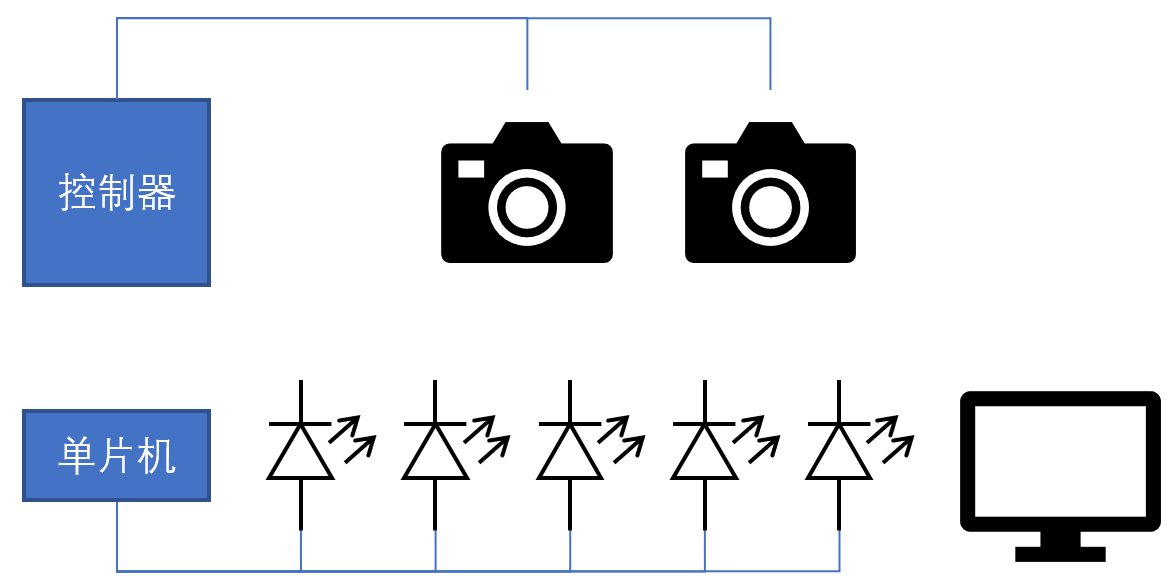
\includegraphics[width=\textwidth]{figures/passive_sync_test}
    \caption{测试过程示意图}
\end{subfigure}%
\begin{subfigure}[b]{0.44\textwidth}
    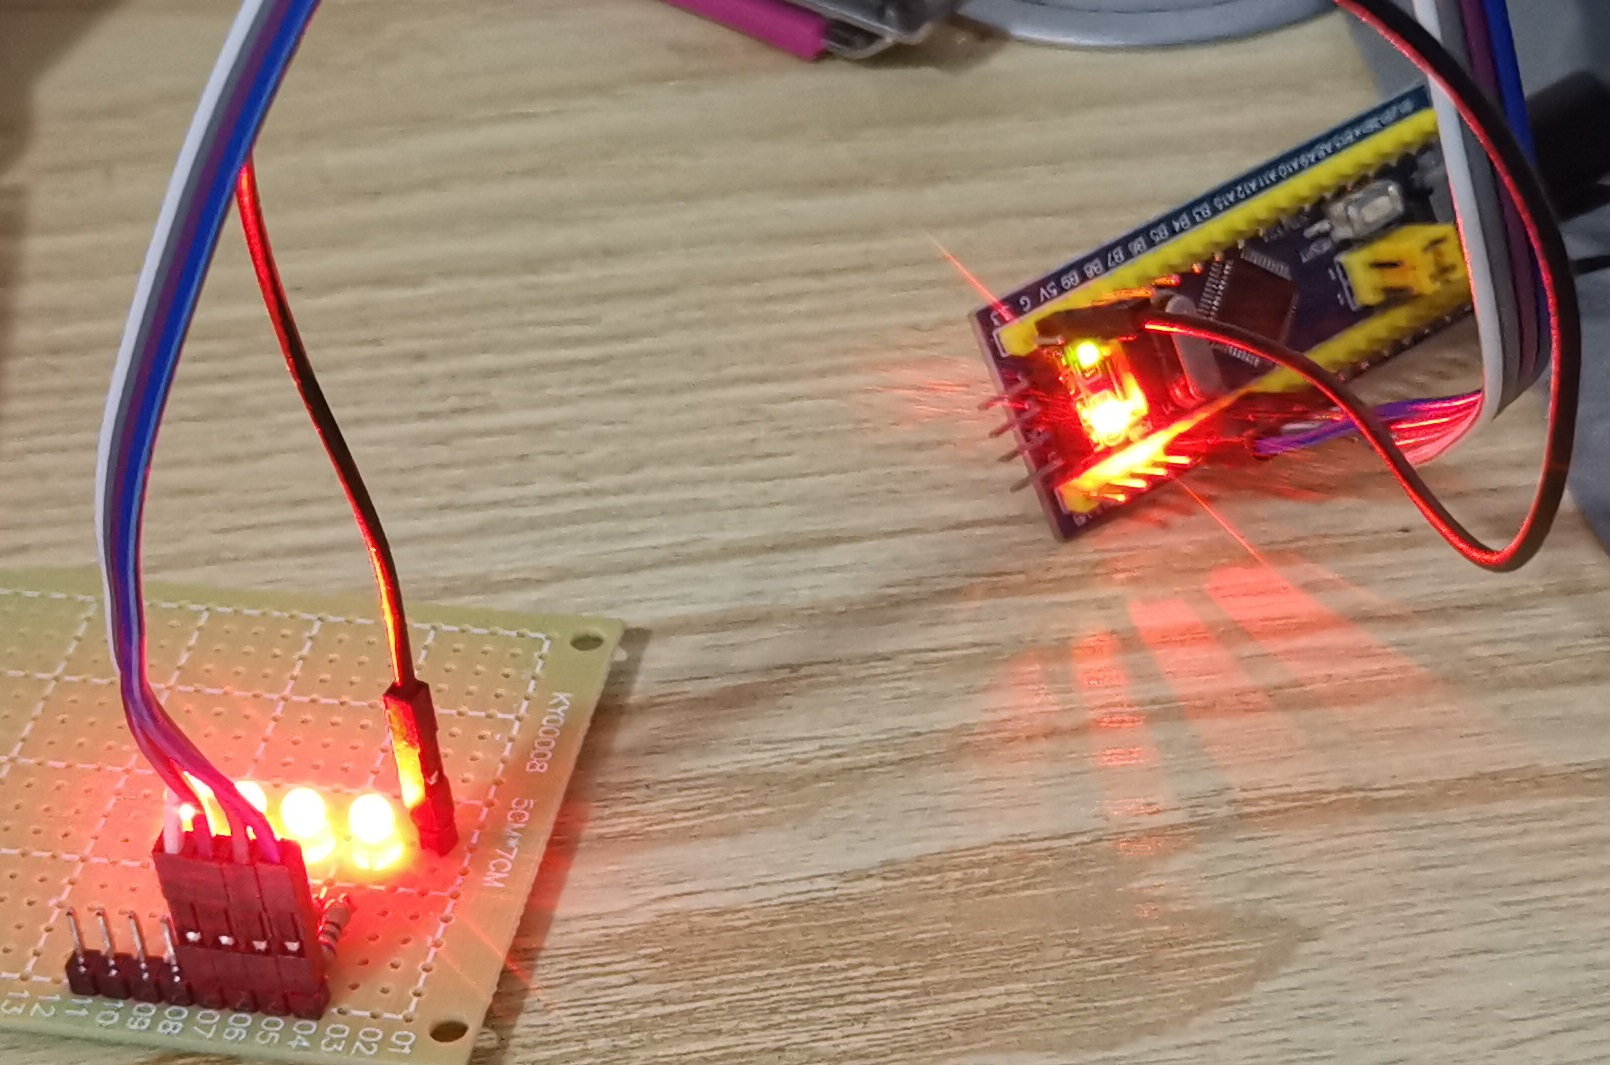
\includegraphics[width=\textwidth]{figures/LED_array}
    \caption{单片机和LED阵列}
\end{subfigure}%
\caption{同步精度测试装置}
\label{fig:passive_sync_test}
\end{figure}

电场的传播速度非常快,因此,当控制器的按钮被按下时,理论上控制信号能同时送达所有相机。
为了实际测试该装置的效果,本文进行了端到端的同步精度测试。
如图\ref{fig:passive_sync_test}所示,该测试的拍摄目标包括5个由单片机控制的LED灯,以及一个60Hz刷新率的显示器(此处使用iPad)。
其中单片机通过硬件计时器中断精确控制LED灯,每个LED灯的亮灭切换间隔依次为0.5ms、1ms、2ms、4ms、8ms,每16ms这些LED灯的状态完成一次循环。
显示器则显示一个秒表,用于判断16ms以上的时间间隔。
然后使用两台相机分别对该测试目标进行拍摄,根据照片中的LED灯状态和秒表的时间,可计算两台相机快门触发时的相对时间。

相机摆放时,需要使LED灯在不同相机传感器的同一位置成像,以避免滚动快门的影响。
拍摄前,需要将快门速度调整为最快的1/4000秒,以尽量避免相机曝光过程与LED的亮灭切换过程重叠,影响读取LED灯的状态。
测试时,将两台相机连接在控制器上,然后多次使用控制器触发快门。
读取结果时,首先丢弃难以判断LED灯状态的图像,
对剩余图像以二进制编码的形式记录LED灯的状态以及屏幕显示的秒表的时间。
对比同一次快门中不同相机拍摄到的照片中读数即可准确获得两台相机曝光的时间差,即控制器的同步精度。

实验结果显示,同时触发快门时,多台佳能R6相机间的同步精度小于0.5ms,即每次拍摄中不同相机的读数均相同。该精度已经足够满足实际应用的需求,且已经远高于快门滚动的速度。
因受到相机最高快门速度的限制,未能以更高的精度完成测试。
此外,本文也测试了R6和另一台佳能90D单反相机间同步的精度,结果显示两台相机间有4ms但非常稳定的延迟。

\subsection{相机标定实例可视化与精度分析}

\begin{figure}
    \begin{minipage}{0.38\textwidth}
        \centering
        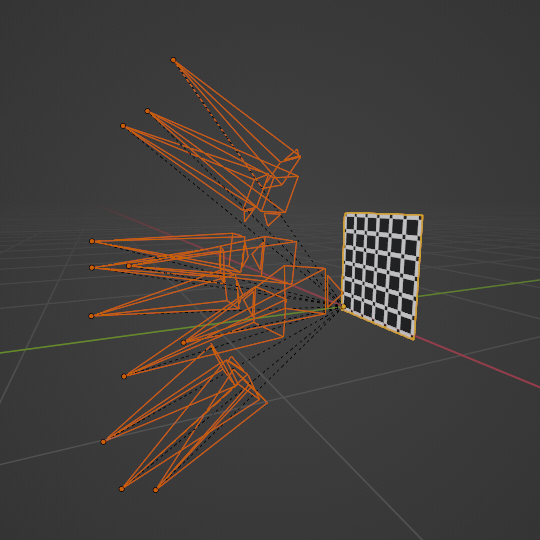
\includegraphics[width=\textwidth]{figures/calib_vis}
        \captionof{figure}{相机标定结果在Blender中的可视化}
        \label{fig:calib_vis}
    \end{minipage}\hfill%
    \begin{minipage}{0.56\textwidth}
        \centering
        \import{build/figures/}{stab_ablation.pgf}
        \captionof{figure}[不同相机的重投影误差]{同一次标定中不同相机第一阶段的重投影误差。其中,10号相机开启了光学防抖,其余相机关闭了光学防抖。}
        \label{fig:stablize_ablation}
    \end{minipage}%
\end{figure}
在标定完成后,本文将最终相机参数和标定板位置导出为glTF格式,以便在Blender等专业3D建模软件中进行可视化。
如图\ref{fig:calib_vis}是本实例的标定结果在Blender中的可视化界面。

然而,可视化只能提供一个直观的感受。本节将进一步对标定的精度进行量化分析,并列举可能影响标定精度的因素。
由于本文采用的相机投影模型参数量小,且角点数量多(约15000个),基本没有过拟合的风险。
因此本文并未单独划分验证集,而是直接使用所有的角点的重投影误差作为标定精度的评价标准。
平均重投影误差定义为:
\begin{equation}
    \label{eq:reproj_err}
    \frac{1}{\|O\|}\sum_{(i,j,k)\in O}\left\|\cornerpix_{i,j,k} - \pi\left(\camparam_i, T_j(\cornerboard_k)\right)\right\|_2
    \text{,}
\end{equation}
其中,$O$为所有可用角点集合。注意该指标与公式\eqref{eq:calib_opt}中的目标函数有所不同,该指标是所有角点的重投影误差的算术平均,以便于进行下文中的各种统计。
上述方法最终获得的平均重投影误差为0.38像素。
以下将对可能影响标定精度的各个因素进行分析:

\paragraph{自动对焦}
由于现实中的相机不是理想的针孔相机,仅有处于焦平面上的物体能清晰成像。
为获得清晰的照片,相机通常默认会开启自动对焦。即通过电机驱动镜片移动,以改变焦平面的距离。
但不幸的是,镜片的移动同样也会导致相机的成像参数发生较大变化,从而无法达到较高的标定精度。
在实践中,若开启了自动对焦,我们则无法获得优于5像素的重投影误差。
因此,在标定和采集数据时设置手动对焦是非常必要的。

\paragraph{光学防抖}
为尽量避免相机机身震动引起的运动模糊,本文使用的镜头配备有光学防抖功能。该功能的原理也是通过电机驱动镜片运动以抵消相机机身的运动的影响。
但是即使本文中的相机是固定在支架上的,光学防抖功能仍然会导致外参的轻微变化。
如图\ref{fig:stablize_ablation}所示,图中仅10号相机开启了防抖,而其重投影误差超出了其他相机近一倍。
因此,关闭光学防抖将有助于提高标定精度。但需注意,关闭防抖后,每次物理接触相机调节参数等之后,再次拍摄前均需要等待5-10秒,以允许整个支架系统恢复稳定。

\begin{table}
    \centering
    \caption[相机畸变模型对标定精度的影响]{
        OpenCV中实现的各种相机畸变模型对标定精度的影响
    }
    \begin{tabular}{l|rr}
        \toprule
        畸变模型(参数数量) & \shortstack{集束调整前\\重投影误差(像素)} & 重投影误差(像素) \\
        \midrule
        无畸变 (0) & 20.220 & 7.011 \\
        默认 (5) & 0.917 & \textbf{0.455} \\
        rational (8) & 0.762 & 0.462 \\
        thin prism (12) & 1.314 & 0.445 \\
        tilted (14) & 0.744 & 0.449 \\
        \bottomrule
    \end{tabular}
    \label{tab:distortion}
\end{table}

\paragraph{相机畸变模型}
相机镜头会带来少量畸变,从而使成像结果与理想的针孔相机成像结果有所差异。
本方案使用了OpenCV中默认的具有5个参数的畸变模型,以建模这种差异。
表\ref{tab:distortion}展示了使用不同畸变模型时重投影误差。
加粗数字为本文最终使用模型。该结果中未排除误差较大的角点。
可见本文所使用的相机具有不可忽视的镜头畸变,对畸变进行建模可大幅提高标定精度。
另一方面,使用更为复杂的畸变模型则没有明显的优势。

\begin{figure}[tbh]
    \centering
    \import{build/figures/}{corner_fit.pgf}
    \small
    \null\hfill
    (a) 不同标定板角度下的精度对比\hfill\hfill
    (b) 不同失焦模糊下的精度对比\hfill\hfill
    (c) 不同噪音下的精度对比\hfill\null

    \caption{OpenCV与本文使用的角点定位算法的精度对比}
    \label{fig:corner_fit}
\end{figure}

\begin{figure}[tbh]
    \centering
    \begin{subfigure}{1.57in}
        \import{build/figures/}{corner_gain-14_0023_opencv.pgf}%
        \caption{OpenCV,增益$2^{14}$}%
    \end{subfigure}%
    \begin{subfigure}{1.57in}
        \import{build/figures/}{corner_gain-10_0023_opencv.pgf}%
        \caption{OpenCV,增益$2^{10}$}%
    \end{subfigure}%
    \begin{subfigure}{1.57in}
        \import{build/figures/}{corner_gain-14_0023_saddle.pgf}%
        \caption{本文,增益$2^{14}$}%
    \end{subfigure}%
    \begin{subfigure}{1.57in}
        \import{build/figures/}{corner_gain-10_0023_saddle.pgf}%
        \caption{本文,增益$2^{10}$}%
    \end{subfigure}%
    \caption[较严重失焦时的角点定位结果]{
        较严重失焦时的角点定位结果。
        图中的红色圆点表示100次随机初始化的收敛位置,
        绿色点表示角点位置真值。
    }
    \label{fig:corner_blur}
\end{figure}

\paragraph{角点定位算法}
角点定位的精度是决定标定精度的关键因素。
为验证本文所实现的算法的性能,本文使用Blender的Cycles渲染器生成了1000张的标定板角点的图像,
这些角点具有随机的位置、角度、失焦模糊和噪声,
并在这组图像上将本文所实现的算法和OpenCV的cornerSubPix算法进行了对比。
具体方法是使用同样的半径$r=15$,使用不同算法分别在每张图像的角点真值附近$10\times 10$像素的范围内随机初始化100次,并优化到收敛,然后统计每张图像的平均重投影误差。
如图\ref{fig:corner_fit}所示,
渲染图像中的噪声服从柏松分布,
增益表示在传感器取得最大读数时接收的电子数量,增益越高,噪声越小。
在Blender渲染的全部1000张图像中,
(a)展示了增益$2^{14}$时距离焦平面-0.3至0.2米的图像中,误差与标定版角度的关系;
(b)展示了增益$2^{14}$时倾斜角度70°以下的图像中,误差与失焦模糊程度的关系;
(c)展示了距离焦平面-0.3至0.2米且倾斜角度70°以下的图像中,误差与噪音强度的关系。
本文在整体精度上大幅优于OpenCV的算法,且在应对极端角度,失焦模糊,随机噪声这些采集中经常出现的情况也有较高的鲁棒性。
而OpenCV的算法在较严重的失焦时则无法正确收敛(如图\ref{fig:corner_blur}),
在相同的半径参数下,本文所实现的算法可处理更大的失焦程度。

\paragraph{角点定位失败造成的外点}
由于角点被其他物体遮挡,或者受到其他物体投下的阴影影响,偶尔角点定位会收敛到错误的位置,造成外点。
但这样的点很少,通常在几十个,因此在实践中未观察到对标定精度有显著的影响。
但是,在统计损失函数或平均重投影误差时,排除这些点可使所得统计数据更能代表整体标定精度。

\begin{table}
    \centering
    \caption{不同后处理方案对标定精度的影响}
    \begin{tabular}{l|rrrr}
        \toprule
        图像源 & \shortstack{定位成功\\角点数} & 离群点 & \shortstack{平均重投影误差\\(像素)}& \shortstack{中位数重投影误差\\(像素)} \\
        \midrule
        原始图像(本文) & 14579 & 21 & 0.4250 & 0.3634 \\
        相机JPG预览图   & 14589 & 18 & 0.4138 & 0.3518 \\
        佳能DPP后处理   & 14592 & 16 & 0.4120 & 0.3515 \\
        \bottomrule
    \end{tabular}
    \label{tab:camera_postprocess}
\end{table}

\paragraph{相机后处理}
数码相机为呈现更加视觉友好的图像,会对采集的数据进行一系列后处理,如去马赛克,gamma映射、降噪、锐化、白平衡等。
为验证这些功能对标定精度可能的影响,本文对比了使用处理前和处理后的数据标定的重投影误差,如表\ref{tab:camera_postprocess}所示。
表中离群点为重投影误差大于3像素的点,这些点在集束调整和数据统计时被排除。
其中后处理使用的是佳能Digital Photo Professional软件,并在默认设置的基础上开启了数码镜头优化,未开启镜头畸变校正,并统一了所有照片的白平衡设置,最终导出为16位TIFF格式图像以保留尽可能高的精度。
它处理一张图片需要约30秒,每次标定采集的数百张图片来说需要耗费的时间相当可观。
此外,本文还对比了相机自动嵌入在原始数据文件中的一张JPG格式的预览图。
结果显示,后处理能略微提升标定精度,并将重投影误差降低0.01像素。使用DPP软件后处理则与预览图相当。
在后处理过程中,佳能可以利用相机和镜头制造的信息以优化结果。
然而佳能的后处理算法并不公开,因此为了保持全流程的可控,且考虑到提升幅度不大,本方案依然选择了使用原始图像进行标定。

\subsection{光源标定实例}

本节通过一个实例展示了本方案中光源标定的实施过程和结果。

本方案利用多张曝光不同的照片合成HDRI。
\begin{figure}[tbh]
    \centering
    \import{build/figures/}{HDRI_stats.pgf}
    \caption[HDRI输入照片读数统计]{HDRI输入照片读数统计。
    (a)中背景的直方图表示照片中像素数量的分布。
    }
    \label{fig:HDRI_stat}
\end{figure}
如图\ref{fig:HDRI_stat}a展示了其中相邻的一对照片的读数对应关系,
可见在超出量程前两张照片的像素值具有很好的线性关系,但通过曝光时间估计的亮度比例与实际有明显偏差。
这说明了本方案的多帧合成方案的合理性,以及通过数据拟合亮度比例的必要性。

有趣的是,虽然理论上ISO越高则噪声水平将越高,但本方案使用的相机在ISO从200增加至400时噪声水平却无明显上升,反而是黑场由512上升到了2048。由此可以推测或许相机在这两种不同配置时处于不同的工作模式。
本方案直接从数据中测量噪声水平,因此可以适应不同的相机配置。

\begin{figure}
\begin{tikzpicture}
    \node [inner sep=0pt, anchor=north west] at (0,0) {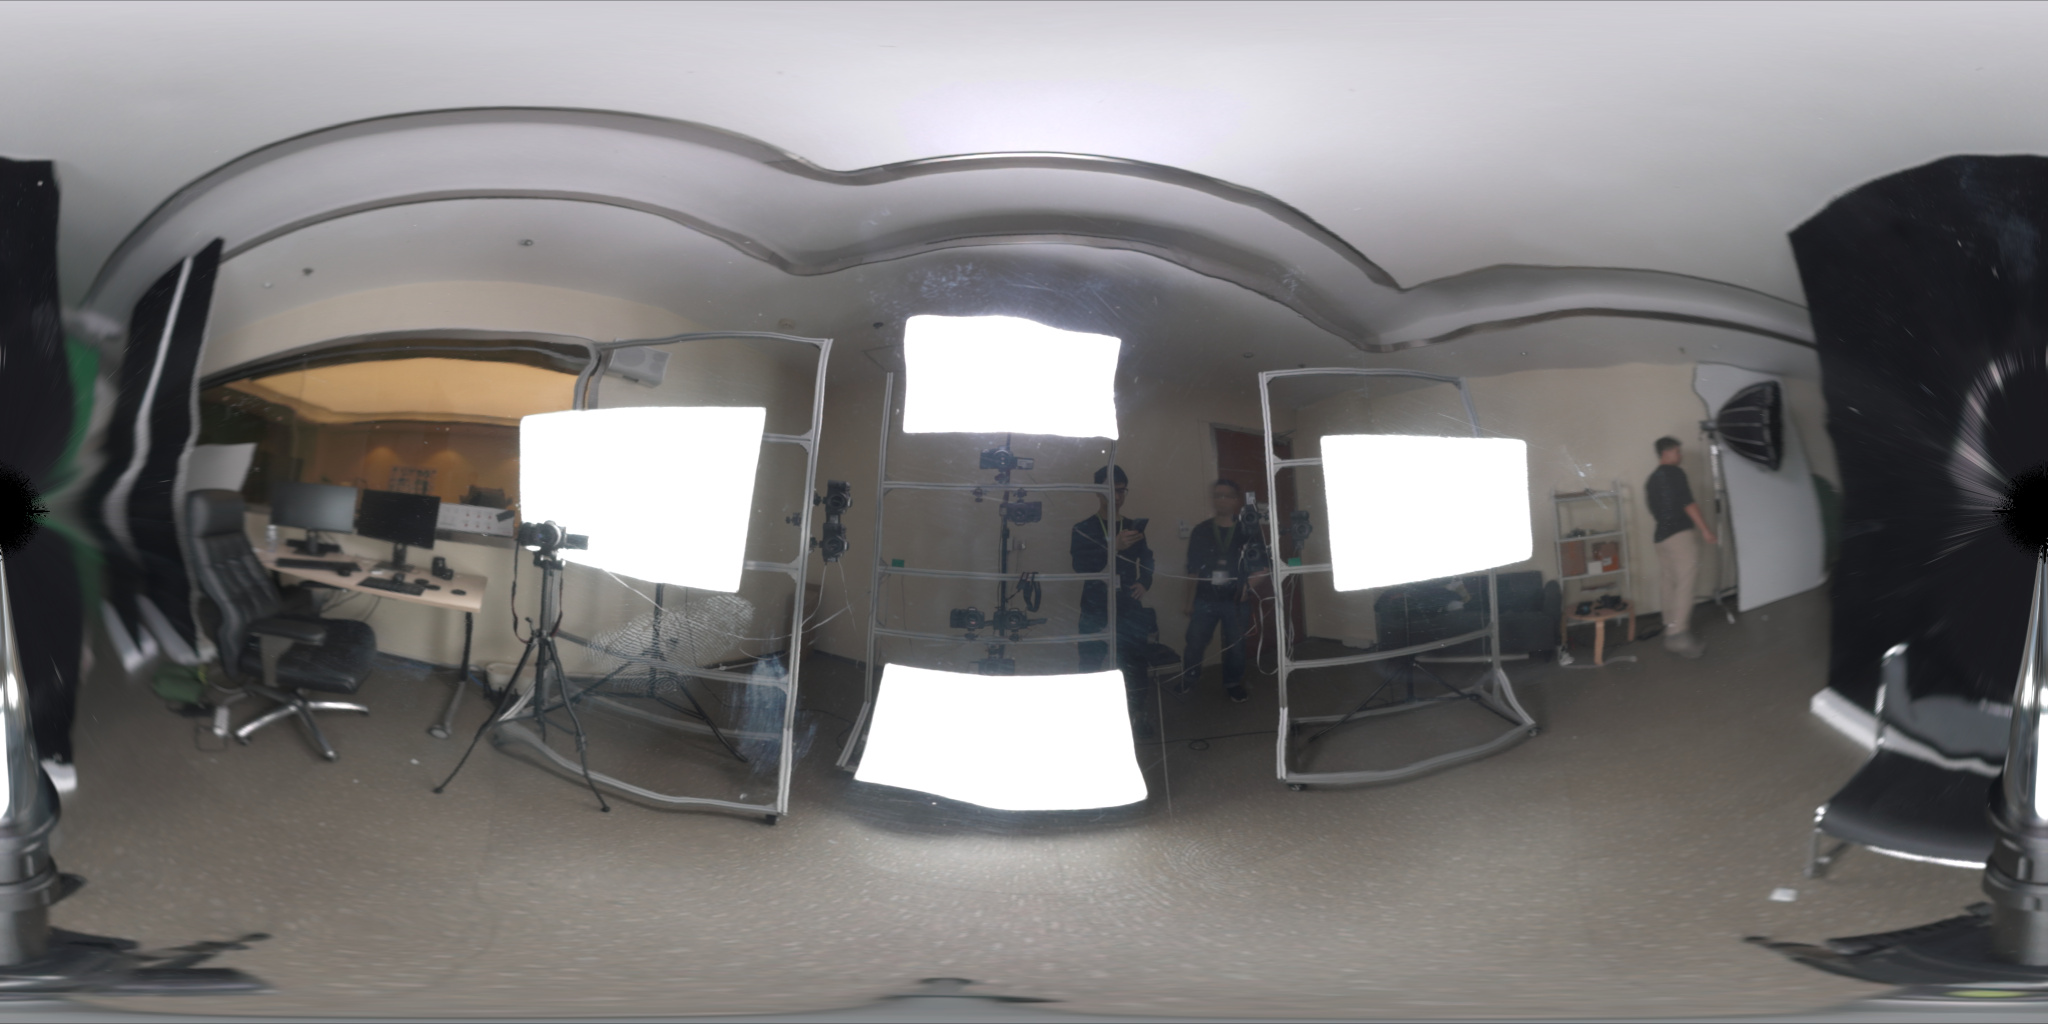
\includegraphics[width=\textwidth]{figures/HDRI}};

    \def\w{4096}
    \node [inner sep=0pt, anchor=north west] (part) at (8.5cm,-0.8cm) {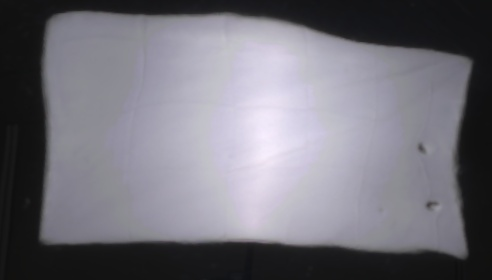
\includegraphics[width=0.1201171875\textwidth]{figures/HDRI_light_part}};
    \coordinate (a) at ({(1768/\w)*\textwidth},{(-620/\w)*\textwidth});
    \coordinate (b) at ({(2260/\w)*\textwidth},{(-900/\w)*\textwidth});
    \node [inner sep=0pt, anchor=north west, draw=red, fit=(a) (b)] (light) {};

    \path [->] (light) edge [red] node [left] {/32} (part);

\end{tikzpicture}
\caption[实验环境全景HDRI]{实验环境全景HDRI。小图展示了其中一个柔光箱处亮度调整到1/32时的图像。}
\label{fig:HDRI}
\end{figure}
图\ref{fig:HDRI}即为使用本方案生成的等距柱状投影格式的环境光照贴图。
该图记录了本文目前实验环境。
从图中可见该图正面质量较好,但背面则有明显变形,精度和分辨率均较低,这是由于背面区域在反射球照片中对应的面积较小。
被反射球本身挡住的一小片区域则完全是黑色。
画面中的局部有一些扭曲,这可能是因为所使用的反射球并不是完美的球形导致的。
未来可通过对反射球的几何形状进行更精细的建模来改善该问题。

\section{后续工作}

以上方案经过验证可以在准确的时间、位置、光照条件下采集到高质量的人脸数据。
后续的研究者们将能基于该方案输出的数据开展诸多人脸重建相关研究,例如:
\begin{itemize}
\item 在传统计算机视觉重建的几何形状的基础上,利用可微分渲染算法,实现符合基于物理的渲染(PBR)流程的人脸材质,包括粗糙度、次表面散射等参数。
\item 利用所采集到的HDRI光源信息,基于分离求和近似(split sum approximation)的可微分光栅化渲染算法,直接端到端地同时估计人脸的几何结构和材质。
\item 利用光线追踪方法,进一步考虑全局光照,以估计更加准确的材质参数。
\item 若将本方案所使用的消费级微单相机更换为工业相机,以实现视频帧同步,则可将其应用于采集人脸动态表情数据。
\end{itemize}

\section*{本章小结}

为解决高精度人脸数据采集环境要求高,实施困难的问题,
本章介绍了一套多视角人脸数据采集方案。
该方案尽量利用市面上可购买的部件,
可支持使用被动光源和主动光源的人脸多视角图像采集。
基于完全受控的全流程数据处理管线,该方案能在准确的时间触发相机快门,
并能输出准确的相机参数、位置和环境光照信息。
本章详细介绍了该方案的软硬件设计,其中硬件包括定制的相机支架,主动和被动同步装置;
软件包括主动同步控制器的单片机固件,光源标定、相机标定、以及一些提升效率的小工具。
这些部分有机结合成了一个精确、高效且灵活可扩展的采集方案。
本章还介绍了该方案各个部件的实现和各个环节的验证。
最后,本章对本方案采集的数据后续可能的利用方式做了展望。
